\chapter{Defensive Points-To Analysis}\label{chapter:defensive}
%Defensive Points-To Analysis: Effective Soundness via Laziness

\epigraph{You don’t just give up. You don’t just let things happen. You make a stand!}{\textit{Rose Tyler} - Doctor Who}
%\epigraph{Progress isn't made by early risers. It's made by lazy men trying to find easier ways to do something.}{\textit{Robert Heinlein}}



%% Static program analysis is an established research area, with a
%% history tracing back to several decades and applications in virtually
%% all modern programming technologies. Static analysis attempts to
%% answer questions about program behavior under all possible inputs.
%% Therefore, virtually all interesting static program analysis questions
%% are undecidable---indeed the prototypical undecidable problem, the
%% \emph{halting problem}, is a static program analysis question: will a
%% program terminate under all inputs?

%% Since static analysis attempts to solve undecidable problems,
%% practical analysis algorithms are of one of two categories: either the
%% analysis intends to under-approximate the precise answer, in which case
%% it is called a \emph{must-analysis}, or it intends to over-approximate
%% the precise answer, in which case it is called a \emph{may-analysis}.

%% The concept of \emph{soundness} (often colloquially used as a synonym
%% of ``correctness'') similarly depends on the flavor of analysis. A 
%% may-analysis is \emph{sound} if it guarantees to over-approximate
%% program behavior, i.e., to capture \emph{all feasible behaviors}. A
%% must-analysis is \emph{sound} if it guarantees to under-approximate
%% program behavior, i.e., to capture \emph{only behaviors certain to
%% be feasible}.

\emph{Soundness} is a coveted property of static analyses, to the
extent that the term is often colloquially used as a synonym for
``correctness''. For a may-analysis, soundness means that the analysis
abstraction overapproximates all concrete executions. A sound
value-flow or points-to analysis is one that computes, per program
point or per variable, value sets that represent (at least) all values
that could possibly arise at the respective point during any possible
execution.

Full soundness is hard to achieve in practice due to code that cannot
be analyzed (e.g., dynamically generated/loaded code, binary/native
code) or dynamic language features (e.g., reflection, \code{eval},
\code{invokedynamic}). We collectively refer to such features as
\emph{opaque code}. For instance, the Java code below invokes an
unknown method, identified by string \code{methodName}, over an
object, \code{obj}.

\vspace{-3mm}\begin{minipage}[l]{5.1in}
\begin{javacodeNoLines}
Method m = obj.getClass().getMethod(methodName);
m.invoke(obj);  
\end{javacodeNoLines}
\end{minipage}

\noindent String \code{methodName} could be a true run-time value---e.g., read
from a file or external resource. Object \code{obj} could itself be of a
type not available during analysis---e.g., \code{obj} could be obtained
through the network and statically typed using a vague interface or
root-of-hierarchy type.

%% Given the prevalence of static analyses, and especially may-analyses,
%% it is a rather surprising fact that practically \emph{no implemented
%%   whole-program static may-analysis is sound for the majority of
%%   realistic programs}~\cite{article:2015:Livshits}. For instance, no realistic
%% may-point-to analysis computes a true over-approximation of the
%% points-to sets that arise during program execution.

%% This is not to say that no sound analyses exist. For instance,
%% abstract-interpretation-based~\cite{popl:1977:Cousot}
%% approaches, such as Astr\'{e}e~\cite{sas:2007:Delmas}, have long emphasized
%% soundness. However such analyses typically reject most real-world
%% programs wholesale, because of the use of language features that are
%% not supported soundly.  Such features include native (non-analyzable)
%% code, \code{longjmp}/\code{setjmp} in C, dynamic loading, reflection, as
%% well as constructs such as the recent Java \code{invokedynamic}. In the
%% context of this paper, we will collectively refer to these features as
%% \emph{opaque code}.

Faced with such complications, all past analyses that claim soundness
have done so under \emph{a priori} qualifications. Prominently,
abstract-interpretation-based~\cite{popl:1977:Cousot}
approaches, such as Astr\'{e}e~\cite{sas:2007:Delmas}, have long emphasized
soundness. The conceptual form of such a soundness result is as
follows:\footnote{This formulation is due to Xavier Rival of the Astr\'{e}e project
  (e.g., \cite{misc:Xavier}).}

\begin{quote}
  An \(Analysis\) of programs in language \(Lang\) is sound relative to
  language subset \(Lang’\) and executions set \(Exec’\) iff:
  
  \tab \tab \(\forall\) program \(P \in Lang\): \(P \in Lang’ \land e \in Exec' \implies e \in \gamma(Analysis(P))\)
  
  (where \(\gamma\) is the concretization function that maps abstractions in the output domain of \(Analysis\) to concrete executions in a universe \(Exec\), superset of \(Exec'\)).
\end{quote}

The problem with this formulation of soundness is that, although it
yields provable theorems, the \emph{a priori} qualification
excludes virtually all realistic programs. The \(Lang'\) or \(Exec'\)
of published proofs disqualify the vast majority of modern programs
``in the wild''. Language subset \(Lang'\) will typically exclude all
dynamic features (e.g., reflection) and/or executions subset \(Exec'\)
will disqualify all behaviors that are deemed too-dynamic (e.g.,
invoking dynamically-loaded code).  Reflection alone disqualifies
$\sim$80\% of Java programs in the 461-program corpus of the recent
Landman et al. study~\cite{icse:2017:Landman}.

The above issues have led several members of
the static analysis community to proclaim that ``\emph{all published
  whole-program analyses are unsound}''~\cite{article:2015:Livshits}, i.e.,
their soundness guarantee does not apply to realistic programs, and
similarly that ``\emph{[there is not] a single realistic whole-program
  analysis tool [...] that does not purposely make unsound choices}''.
The problem is, therefore, both theoretical and practical. Soundness
theorems do not give guarantees for realistic
programs. Implementations of analyses in tools happily perpetuate the
illusion: they handle soundly the language features one can prove
theorems about, while cutting corners in the sound handling of all
\emph{other} features, in order to demonstrate greater scalability or
precision. For instance, in our earlier Java code fragment, even if
the type of \code{obj} is known, many implemented static analyses will
not consider all its methods (which now form a small finite set) as
possible values of \code{m}, but will instead ignore the code
altogether.  This phenomenon has led to the introduction of the term
\emph{soundy}~\cite{article:2015:Livshits} to characterize such analyses.
Despite the derogatory tone, ``soundy'' analyses are the current
\emph{good} case of static analyses! They are realistic analyses that
handle all ``normal'' language features soundly.

In this work, we propose \emph{defensive analysis}: a static
analysis architecture that addresses the above soundness
shortcomings. The basis of defensive analysis can be seen as a different conceptual
formulation of soundness.

\begin{quote}
  An \(Analysis\) of program \(P\) in language \(Lang\) computes
  results, \(Analysis(P)\), together with soundness marker sets,
  \(Claim(P)\). The \(Analysis\) is sound iff:
  
  \tab \tab \(\forall\) program \(P \in Lang\), execution \(e\): \(e[Claim(P)] \in \gamma(Analysis(P))[Claim(P)]\)
  
  (where \(\gamma\) is as before, and \(e[Claim(p)]\) is the restriction of an execution \(e\) to program points with soundness claims, and the definition is similarly lifted to sets of executions).
\end{quote}

\noindent In other words, the analysis imposes no (or very liberal)
\emph{a priori} restrictions to its soundness claims, but instead
\emph{computes} the claimed domain of its soundness: the program parts
for which the analysis result is sound. The soundness theorem applies
to all (or most) programs, under all execution conditions---instead of
eagerly disqualifying the vast majority of real-world programs. The
extent of soundness is now defined over program points and becomes an
experimentally measurable quantity: the size of \(Claim(P)\) (which we
term the \emph{coverage} of the analysis) can be measured to quantify
for which percentage of a program's points the analysis is guaranteed
to produce sound results.

The challenge of defensive analysis is, thus, to distinguish parts of
the program that are certain to not be affected by opaque
code. Delineating ``safe'' from ``unsafe'' parts of the program is an
ambitious goal, since opaque code can do virtually anything: it can
add dynamically-generated subclasses with never-seen methods that get
called (via dynamic dispatch or first-class functions) at unsuspecting
program points; it can call any existing method or alter any field via
reflection; it can interpose its own implementations at every place
where the program uses a reflective lookup; worst of all, it can wreak
havoc on all parts of the heap reachable from any reference that
escapes into opaque code.

%% To achieve the goal of distinguishing ``safe'' inferences, defensive
%% analysis has a different logical form from past analyses. Instead of
%% adding sophisticated handling of opaque code, defensive analysis
%% redefines the analysis logic for regular, common language features, to
%% defensively protect against the possibility that the analysis
%% information potentially depends on opaque code. In essence, a
%% defensive analysis produces inferences only when these are guaranteed
%% to hold because of existing code and language features, and cannot
%% possibly be violated by other, unknown code. Although this seems like
%% a straightforward mode of operation, applying it to yield a realistic
%% static analysis with useful coverage is a challenge.

We designed and implemented a defensive may-point-to (henceforth just
``points-to'') analysis for Java. The analysis follows the above form,
explicitly designating points-to sets that are sound, i.e., that contain
at least all the values that may ever arise in actual executions. Soundness
guarantees carry over to the implementation: the soundness proof
explicitly models all other language features as \unknowninstr{}
instructions and makes only weak, semantically-justified assumptions
(e.g., a type-safe heap) about them. Soundness reasoning is defensive
in that it establishes when the analysis can be certain to know the
full contents of a points-to set, no matter what opaque code can do
(within the stated weak assumptions).

In our effort to implement defensive analysis in a realistic package,
we found \emph{laziness} to be an essential feature---the analysis
cannot scale without it for real-world programs. Laziness means
that the analysis does not compute points-to sets unless it can also
claim their soundness. That is, program points outside of the
\(Claim(P)\) set do not get populated at any point---they remain empty
throughout the analysis.  Consequently, all points-to sets with a
potentially unbounded number of objects (e.g., sets that depend on
reflection or dynamic loading) are represented as the empty set: the
analysis never computes any contents for them. An empty analysis
result merely means ``I don't know'', which could signify that the
points-to set is affected by opaque code, or simply that the analysis
cannot establish that it is \emph{not} affected by opaque
code. Laziness yields high efficiency: the analysis can fall-back to
an empty set (i.e., implicitly unbounded) without performing any
computation or occupying space.

%% That is, when the analysis infers that a variable
%% can point to \emph{anything}, it assigns it an empty points-to
%% set. This choice may at first seem rather counter-intuitive, but it
%% yields several significant advantages.  First, the approach acquires
%% an intuitive interpretation if one views empty points-to sets as
%% signifying ``don't know''/''cannot bound'' values: an empty set simply
%% implies that the analysis has failed to upper-bound its
%% % possible
%% contents.
%% %, which is a rather natural interpretation. 

The defensive nature of the analysis combined with laziness result in
a very simple specification. The analysis does not need to integrate
complex escape or alias reasoning (i.e., ``can this object \emph{ever}
escape into opaque code?''), but only best-effort logic (i.e., ``here
are simple, safe cases, when the object cannot possibly be affected by
opaque code''). Failure to establish non-escaping merely means that
the points-to set remains empty, to denote ``I don't know'' or
``potentially unbounded''.

%In fact, a
%property of our analysis is that points-to sets become non-empty only
%when there is a guarantee that all sources of their values have been
%identified and are bounded.

%compact points-to sets, since
%unbounded ones are over-approximated \emph{implicitly} (i.e., without
%an explicit enumeration of their contents).

%Third, the approach allows
%the analysis to never ``waste work'': no values enter a points-to
%set if they will later be overwritten (because the points-to set will be found to be
%unbounded).
%core of the analysis logic to be self-evidently monotonic, significantly
%simplifying reasoning.

%% In terms of applications, soundness is a requirement for
%% ambitious clients, such as automatic optimization or 
%% semantics-preserving refactoring. Such clients are simply not
%% feasible with past approaches.
%% %% SPACE
%% %with prior analysis approaches.
%% In particular, inter-procedural automatic optimization has long been
%% hindered by the absence of sound points-to analysis information. Thus,
%% our work has significant potential for wide practical application.

\noindent Concretely, the work makes the following contributions:

\begin{itemize}
\item We offer a general static may-point-to analysis that
  yields sound results for realistic programs in the presence of
  opaque code.
  %% (Arguably other approaches
  %% \cite{ecoop:2004:Hirzel,article:2007:Hirzel,pldi:2007:Lattner} achieve
  %% soundness, but not for the full problem. Additionally, an analysis
  %% can be nominally sound by rejecting wholesale any program that
  %% employs features that the analysis does not handle. This is also not
  %% a solution. We compare more thoroughly in the related work section.)

%% \item The analysis has a simple, yet effective, form.  It starts from
%%   a sound state: all points-to sets are empty, denoting ``potentially
%%   unbounded''.  It can then build from the ground up, i.e., to only
%%   reason about known safe cases. More sophisticated machinery (such as
%%   expensive escape or alias analysis) can grow the set of these safe
%%   cases, but is not a prerequisite for soundness.  The analysis is
%%   also modular: it can be applied to any subset of the program, and
%%   will merely leave more points-to sets empty if other parts are
%%   unknown.

\item The analysis is efficient, leveraging its lazy representation of
  points-to sets. As a result, it can be made precise, beyond the
  limits of standard whole-program points-to analyses---e.g., for a
  5-call-site-sensitive and flow-sensitive analysis. The analysis is
  also modular: it can be applied to any subset of the program, and
  will merely leave more points-to sets empty if other parts are
  unknown.
  
\item We show that the analysis, though quite defensive, yields useful
  coverage. In measurements over large Java benchmarks, our
  analysis computes guaranteed over-approximate points-to sets (\(Claim(P)\)) for
  34-74\% of the local variables of a conventional unsound analysis.
  (This number is much higher than that of a
  conventional sound but intra-procedural analysis.)  Similar
  effectiveness is achieved for other metrics (e.g., number of calls
  de-virtualized), again with actionable, guaranteed-sound
  outcomes.

%%   Finally, the analysis is efficient,
%% %and precise, 
%%   due to its tight representation of points-to sets: we evaluate
%% %a setting of 
%%   a highly precise flow-sensitive, 5-call-site-sensitive defensive
%%   analysis, which would be too heavyweight for typical past approaches.

%% \item The work brings some clarity to the domain of static analysis of
%%   opaque code. The approach allows, for the first time, to
%%   quantitatively weigh the benefits of sound inter-procedural analysis
%%   against its costs.

  %% SPACE
%  and decide whether unsoundness is tolerable, or a
%  fully sound approach is preferable.
\end{itemize}



\section{Analysis Illustration}
\label{sec:illustration}

We next describe the setting of defensive analysis and illustrate its
principles and behavior.


\subsection{Soundness and Design Decisions Overview}

Defensive analysis is a may-point-to analysis based on access
paths, i.e., expressions of the form ``\args{var}(.\args{fld})*''.
That is, the analysis computes \emph{the abstract objects} (i.e.,
allocation sites in the program text) \emph{that an access path may
  point to}. The analysis is \emph{flow-sensitive}, hence we will be
computing separate points-to information per program point. Both of these
design decisions are integral elements of the analysis, as we will
justify in Section~\ref{sec:principles}.

Soundness in this setting means that the analysis computes an
over-approximation of any points-to set---i.e., the analysis computes
(abstractions of) all objects that may occur in an actual
execution. However, since not all allocation sites are statically
known (due to dynamically loaded code), such an over-approximation
cannot be explicit: not all possible values in a points-to set can be
listed.  Thus, there needs to be a special value, $\top$, to denote
``unknown'', i.e., that the analysis cannot bound the contents of a
points-to set.

Defensive analysis takes the above observation one step further, by employing a
\emph{lazy} approach: it never populates a points-to set if it cannot
guarantee that it is bounded. Thus, an empty points-to set for an
access path signifies that (as far as the analysis knows) the access
path can point to anything.\footnote{We use an explicit abstract value
  for \texttt{null}, therefore a points-to set that only contains
  \texttt{null} is not empty. This is standard in flow-sensitive
  analyses, anyway. (In flow-\emph{in}sensitive analyses,
  \texttt{null} is typically a member of every points-to set, so it is
  profitable to not represent it, and hence have an empty set mean a
  \texttt{null}-only reference. No such benefit would arise in our
  flow-sensitive setting.)}

In other words, an empty set can be thought to
represent a bottom ($\bot$) value during the analysis computation: it
just marks a set as having no known values (yet). A set stops being empty
only when all the possible ways (in known or unknown code) to contribute
values to it have been examined and are found to have bounded contents.
At the end of the analysis, all sets that have remained empty
signify that the analysis could not bound their contents, i.e., they
do not belong in the set \(Claim(P)\) of program points with
soundness claims. Therefore an empty set after termination of
the analysis is conceptually equivalent to a top ($\top$) value: the
set could contain anything. This is consistent with the defensive
nature of the analysis: not knowing all the values of a set is considered
just as bad as knowing it can point to anything.

%% since the analysis is defensive, there is no need to
%% distinguish a $\top$ value from a $\bot$ (empty) value: not knowing
%% the values of a set (i.e., a $\bot$ value) is just as bad as
%% knowing it can point to anything ($\top$). One can
%% think of the analysis as lazily keeping points-to sets at $\bot$
%% until they get concrete, bounded contents. Then, at the end of the
%% analysis, sets that stayed $\bot$ are reported as $\top$, i.e.,
%% unbounded.

With this representation choice, the analysis does not need to expend
effort in order to be sound. All points-to sets (for any valid access
path, of any length) start off empty, i.e., if the analysis were to
stop at that point it would report them as having $\top$ values,
meaning ``the set can contain anything''. This is a sound answer, and
is only subsequently refined.
%Defensive analysis conservatively keeps
%a set empty until it has enough information to compute finite contents
%for it.
%However, having an
%explicit value for $\top$ is detrimental to an actual
%implementation.

This lazy evaluation means that defensive analysis does not need to
employ sophisticated mechanisms to simply be sound. For instance,
instead of a precise over-approximate escape
analysis,
%(which will avoid over-computing objects that escape into opaque code,
%so as to avoid invalidating all possible points-to sets by adding
%$\top$ values),
defensive analysis can use a simple analysis
(including none at all) to compute straightforward cases when an
object is guaranteed to never escape into opaque code.

%% In this way, the analysis reasoning does not proceed by ``computing
%% $\top$ values when a points-to set could potentially be influenced
%% by opaque code'' but by ``computing finite, non-empty points-to sets

%% Since all points-to sets are empty by default, representing them
%% lazily, as empty sets, requires no computation and no storage. This may
%% seem like a small matter (zero bits vs. one bit)


%% The key principles of defensive analysis, however, are to maintain a
%% simple specification and maximum efficiency. In line with the
%% simplicity principle, the analysis should not be highly sophisticated
%% just to be simply sound.


%% In defensive analysis, ``not knowing that a set is
%% bounded'' produces the same final result ($\top$) as ``knowing that
%% the set is not bounded'' (e.g., computed via reflection).


%In other words, a points-to set
%remains empty ($\top$) until the analysis can guarantee that the set's
%contents will be finite, i.e., that the set will not be $\top$. Once a
%set stops being empty, it never reverts to empty.


%
%Instead, our implementation of defensive analysis uses the
%\emph{empty set} to represent $\top$.


\subsection{Background and Illustrating Design Decisions}
\label{sec:principles}

We can see the rationale behind our design decisions through simple
examples.

\paragraphhead{Baseline intra-procedural resoning.}
It is easy for an analysis to be sound locally, in an
\emph{intra-procedural} setting. For instance, when a
variable is freshly assigned with a newly allocated object,
we are guaranteed to soundly know its points-to set:

\vspace{-3mm}\begin{minipage}[l]{5.1in}
\begin{javacodeNoLines}
x = new A();  // abstract object a1, x points-to set is {a1}
\end{javacodeNoLines}
\end{minipage}

We can also propagate such information transitively through local
assignments (a.k.a. ``move'' instructions), as long as no opaque code
can interfere. In the case of local variables, standard concurrency
models (for Java, C++, etc.) do not allow interference from other
threads, hence points-to sets remain sound, as long as the code
itself does not call out to opaque code:

\vspace{-3mm}\begin{minipage}[l]{5.1in}
\begin{javacodeNoLines}
x = new A();  // abstract object a1, x points-to set is {a1}
y = x;  // y points-to set is {a1}
z = y;  // z points-to set is {a1}
\end{javacodeNoLines}
\end{minipage}

This approach is one often taken by traditional compilers
(ahead-of-time or just-in-time alike) in order to perform
intra-procedural optimizations, such as those based on traditional
data-flow analysis. (Later, in our experimental evaluation, we compare
against such a baseline ``intra-procedural sound'' analysis.)

However, the challenge is to also reason soundly about
\emph{inter-procedural} behavior. This includes reasoning about the
heap (i.e., reading fields of objects) and about method calls and
returns, whose resolution may be dynamic. This will be the focus of
the defensive analysis specification.

\paragraphhead{Inter-procedural elements.}
The large potential for opaque code to affect inter-procedural
analysis results has prevented past analyses from being sound. For
instance, consider a simple heap load instruction:

\vspace{-3mm}\begin{minipage}[l]{5.1in}
\begin{javacodeNoLines}
x = y.fld;
\end{javacodeNoLines}
\end{minipage}

\noindent Imagine that the analysis has (somehow) soundly computed all
the objects that \code{y} may point to. It may also know all the places
in the code where field \code{fld} is assigned and what is
assigned to it. However, the analysis still cannot compute soundly the
points-to set of \code{x} unless it also knows that all objects
referenced by \code{y} can never escape to opaque code. This is
hard to establish: not only do all sites of opaque code
(reflection, unknown instructions, potential dynamic code generation
sites, and more) need to be marked, but the analysis needs to know an
over-approximation of which objects these sites can reach. This
requires to have pre-computed an over-approximate (i.e., sound)
points-to analysis, which is the problem we are trying to solve in the
first place. Past work has dealt with this problem with unrealistic
assumptions. For instance,
%\citet{pldi:2000:Sreedhar}
Sreedhar et al. \cite{pldi:2000:Sreedhar} present a
call-specialization analysis that can handle dynamic class loading,
but only if given the results of a sound may-point-to analysis as
input.
%% Any solution along these lines will likely involve a complex
%% interplay between points-to and escape reasoning.

Instead, defensive analysis pessimistically computes that a points-to
set is $\top$ (i.e., can contain anything) unless it is certain that
its contents are bounded. When can the analysis know this, however?
Such a guarantee of bounded contents typically comes from having
precisely tracked the contents of a variable or field all the way from
its last assignment, and having established that no other code could
have interfered.  For instance, let us expand our earlier example:

\vspace{-3mm}\begin{minipage}[l]{5.1in}
\begin{javacode}
y.fld = new A(); // abstract object a1, y.fld points-to set is {a1}
... // analyzable, non-interfering code
x = y.fld;
\end{javacode}
\end{minipage}

The analysis can now know that the points-to set of \code{x} is
\code{\{a1\}}, i.e., the singleton containing the allocation site for
\code{A} objects on line 1. For this to be true, the analysis has to
establish that all code between the store instruction to \code{y.fld}
and the subsequent load does not interfere with the value of
\code{y.fld}. For example, we can be certain of such non-interference if
the code does not contain a store to field \code{fld} of \emph{any}
object, does not call any methods, and no other thread can change the
heap at that segment of the program.% under our concurrency model.
These are simple, local conditions that the analysis may well be able to
establish.

In practice, our defensive analysis will do a lot more: it will track
method calls, up to a maximum context depth, to ascertain when they
can interfere with points-to sets. (If any interference is detected,
the points-to set propagated forward is empty.) For instance, in
the example code below, the analysis can know with certainty the
points-to set of \code{x} on line 6, whenever method \code{foo} is
called from line 3 of the program fragment.

\vspace{-3mm}\begin{minipage}[l]{5.1in}
\begin{javacode}
y.fld = new A(); // abstract object a1, y.fld points-to set is {a1}
z.otherFld = new B();
foo(y);

void foo(W w) {
  x = w.fld;  // x-for-call-site-3 points-to set is {a1}
}
\end{javacode}
\end{minipage}

Note the elements that contribute to such reasoning: The result holds
soundly only when \code{foo} is called from the specific call site. This
result is established only by tracking the value of \code{y.fld}
(renamed to \code{w.fld} inside method \code{foo})
instruction-by-instruction all the way to line 6. The heap store
instruction on line 2 is guaranteed to not affect \code{y.fld} (regardless
of whether \code{z} and \code{y} alias or not), since
Java guarantees object isolation and the reference is to a different
field. (More on language model assumptions in
Section~\ref{sec:assumptions}.)

The above example helps illustrate the design choices of defensive
analysis: it is a flow-sensitive, context-sensitive analysis because
it needs to track all points-to information that is guaranteed to
hold, per-instruction, following closely all possible control-flow of
the program, even across calls. It is also an analysis computing
points-to information on \emph{access paths} because this gives
significantly more ability to reason about the heap locally.  For
instance, in the above program fragment, we may not know which objects
\code{y} may point to.\footnote{In fact, even if we did know, these
  would be abstract objects.  Static analysis would almost never be
  able to establish soundly what their \texttt{fld} field points to,
  because this information needs to capture the \texttt{fld} values of
  all \emph{concrete} objects (not just the latest one)
  %  , but also those allocated long ago)
  represented by the same abstract object.}
%
%  It is near-impossible for an analysis to be sound
%  when computing points-to sets of fields of abstract objects, because
%  these need to include all values that the field of any concrete
%  object would point to. However, the concrete objects 
%
However, we do know that \code{y.fld} certainly points to abstract
object \code{a1} after line 1!


% \subsection{Representing $\top$}

%It is easy to state a defensive analysis theoretically, with $\top$
%values used to designate unbounded points-to sets. 
%Generally, computing a value that essentially
%means ``I don't know'' requires (potentially expensive) computation.


%At every step, the defensive analysis logic has an
%intuitive general form:
%\begin{quote}
%``if we know all sources of values for a points-to set, and if all
%  these sources have bounded points-to sets, then the set is bounded
%  and equal to their union.''
%\end{quote}

%\noindent In our representation this means that a set is non-empty
%only if all of its source sets are guaranteed non-empty.

%We address the above concerns by exploiting the nature of defensive
%analysis: not knowing all the values in a set is equivalent to making
%the set $\top$. We, thus, 

\paragraphhead{Laziness.}
Finally, consider the design choice of representing unbounded
points-to sets as empty, i.e., to lazily compute the contents of
points-to sets only if they can be proven to be finite. Defensive
analysis requires laziness for scalability. (Experimentally, a
non-lazy analysis does not scale for any non-zero context depth, i.e.,
cannot be effective inter-procedurally.)

Laziness means skipping an explicit representation of $\top$, in favor
of keeping points-to sets empy ($\bot$ in the usual lattice of sets)
as long as possible. (As mentioned earlier, at the end of the
analysis, all sets that stayed $\bot$ become implicitly $\top$.)  This
has the minor benefit of avoiding storage of $\top$ values, since
empty sets are represented without consuming memory. More majorly,
however, it enables the analysis to give a convenient meaning to any
finite points-to sets that arise. Instead of ``\emph{this set
  currently has bounded contents, but may become $\top$ during the
  course of the analysis}'', a non-empty set of values implies
``\emph{this set has bounded contents and is guaranteed to always have
  bounded contents}''. By making this distinction, the analysis never
wastes effort computing points-to sets with explicit (non-$\top$)
contents only to later discover that the points-to set is $\top$.  For
an example of how much wasted effort can be saved by being lazy,
consider an example program involving a heap load and a virtual call:
%of a heap load,
%augmented with a virtual call, inside a loop:

\vspace{-3mm}\begin{minipage}[l]{5.1in}
\begin{javacode}
y.fld = new A();  // abstract object a1
while (...) {    
  x = y.fld;
  x.foo(y);
}
\end{javacode}
\end{minipage}

An analysis may have computed all the abstract objects that
\code{y.fld} may point to at line 3. One of these computed objects may
induce a different resolution of the call instruction (line 4), which
can suddenly lead to the discovery that a \code{y.fld}-aliased object
can enter opaque code (while this was not true based on what the
analysis had computed earlier). Since the object referenced by
\code{y.fld} can change in code that is not analyzed, the points-to set
of \code{x} at the load instruction will need to be augmented with the
implicit over-approximation special value, $\top$.  This means that
all previously computed values for the points-to sets of \code{x} and
\code{y.fld} are subsumed by the single $\top$ value. Computing these
values and all others that depend on them constitutes wasted
effort. To make matters worse, this is more likely to happen for
\emph{large} points-to sets, i.e., the more work the analysis has
performed on computing an explicit points-to set, the larger (and less
precise) the set will be, and the more likely it is that the work will
be wasted because the set will revert to $\top$.

%It is, therefore, a key requirement for a defensive analysis to never
%compute explicit points-to sets if these sets will later revert to
%$\top$.

%% Instead, defensive analysis conservatively keeps all sets empty until
%% it has enough information to compute finite contents for them.
%% The analysis incurs cost only when it knows that a result is
%% guaranteed to be bounded. Recall how a defensive analysis needs to
%% track the values of access paths all the way from their last
%% assignment to the current instruction, even through method calls. This
%% kind of precision is possible in practice only because the tracked
%% points-to sets are small---larger sets are conservatively
%% over-approximated with $\top$, i.e., stay empty.

The design principle of ``laziness in order to avoid wasted effort''
is responsible for the scalability of defensive analysis. As we show
in our experiments, defensive analysis scales to be flow-sensitive,
5-call-site sensitive over large Java benchmarks and the full JDK.
%No past may-point-to analysis scales to such context depths.
(In standard past literature for all-program-points analyses, even a
flow-\emph{insensitive}, 2-call-site-sensitive analysis has been
infeasible over these
benchmarks~\cite{pldi:2014:Smaragdakis}.\footnote{It is
  worth emphasizing that, although defensive analysis is lazy, this
  is a very different form of laziness than that of \emph{on-demand}
  points-to analysis (e.g.,
  \cite{ecoop:2016:Spath,popl:1997:Biswas}). An
  on-demand analysis only computes points-to information for program
  points that may affect a particular site of interest, instead of the
  entire program. The defensive analysis we describe is an
  all-program-points analysis: it computes points-to information for
  the entire program, i.e., for all possible points-to queries,
  including ones potentially devised in the future. Yet the analysis is
  lazy in that it only computes values for points-to sets that it can
  prove to have bounded contents.})

%Otherwise, the defensive analysis would be doing most of the
%work of an unsound, conventional may-point-to analysis, before making
%it sound by attaching $\top$ values to unbounded sets. This is not
%practically possible given the precision needs of defensive analysis.
%For instance, our implemented defensive analysis performs a
%flow-sensitive, 5-call-site-sensitive analyses over large benchmarks
%and the full Java library. No past analysis 

%% This representation has the added benefit
%% of allowing the analysis logic to be expressed as simple set unions
%% and intersections, with no negation. In this way, it is trivial to
%% show that the analysis is monotonic. Finally, this makes the analysis
%% inexpensive: an over-approximate result (the empty set) requires no
%% computation.

\subsection{Soundness Assumptions}
\label{sec:assumptions}

The soundness claims of defensive analysis are predicated on
assumptions about the environment. These assumptions reflect well the
setting of safe languages, such as Java:
%% SPACE%%---our implementation setting:

\begin{itemize}
\item \textbf{Object isolation.} Objects can only be accessed via
  high-level references. This means that objects and fields are
  isolated: an object can be referenced outside the dynamic scope of a
  method or by a different thread only if a reference to the object
  has escaped the method or current thread. (This restriction also
  implies that objects are not contained in one another, though they
  can contain references to each other.) A field can only be accessed
  via a base object pointer and a unique field signature.
  
\item \textbf{Stack frame isolation.} Local variables are isolated
  from each other, thread-private and private to their allocating
  method. No external code can access the local variables of a method,
  even if the code is executed (i.e., is a callee) under the dynamic
  scope of the method.

\item \textbf{Concurrency model.} In the simplified model of the
  paper, soundness is predicated on the assumption that standard
  mutexes (or operations on volatile variables) are used to protect
  all shared memory data. We later discuss
%  In Section~\ref{sec:discussion} we discuss
  how our implementation removes this assumption.\footnote{The reason
    for the simplified concurrency model in the paper is that it
    allows presenting the analysis in its purest form, dealing with
    core language features such as heap loads/stores and calls, but
    unencumbered by auxiliary considerations (e.g., computing objects
    that do not escape into other threads).}
\end{itemize}

Thus, our setting is clearly that of a safe language with near-unlimited
potential for dynamic behavior. Notably, we can have unknown
instructions; calls to native code with arbitrary behavior (over a
well-typed, isolated heap); generation and loading of unknown code
(which may also be called, via dynamic dispatch, by unsuspecting
\emph{known} code); arbitrary access to existing or unknown objects
(both field read/writes and method calls) via reflection, i.e.,
without such access being identifiable in the program text; and
more.


\section{Defensive Analysis, Informally}
\label{sec:analysis-informally}

The discussion of analysis principles in the previous sections gives
the main tenets of defensive analysis. However, these need to be
concretely applied over all complex language features affecting
points-to information: control-flow merging, heap manipulation, and
method calls. We give informal examples next. Following these
examples should significantly facilitate understanding the formal
specification of the analysis, in later sections.

%The key principle of defensive analysis is that of computing
%\emph{explicit} points-to sets (i.e., points-to sets with their
%contents enumerated) only when the analysis can statically bound their
%contents.  Bounding the contents of a points-to set means that all
%possible sources of values are known and are also bounded. In all
%cases when a points-to set cannot be bounded, its contents are
%over-approximated implicitly, i.e., the set has the value $\top$.

%The defensive analysis principles have to apply to every deep
%feature of the language: 

\paragraphhead{Control-flow merging.}
Consider a branching example:
%% SPACE
%of two branches and the information at
%their merge point.

\vspace{-3mm}\begin{minipage}[l]{5.1in}
\begin{javacode}
if (complexCondition()) {
  x = new A();  // abstract object a1
   // x points-to set is {a1}
} else {
  x = notFullyAnalyzed();
   // x points-to set is {} 
} // x points-to set is {} 
\end{javacode}
\end{minipage}

The first branch of the above \code{if} expression establishes that the
points-to set of variable \code{x} is \code{\{a1\}}. For a conventional
analysis, this would result in adding \code{a1} to the points-to set of
\code{x} at the merge point (after line 7). The defensive analysis, however,
has to be conservative and not compute values that may later become
$\top$. Therefore, it will add \code{a1} to the final
points-to set of \code{x} only if it can also prove that the points-to
set of \code{x} in the second branch is bounded, i.e., non-empty. If the analysis is not
certain of this, the points-to sets of \code{x}, both in the second
branch and at the merge point, stay empty. Inability to
bound the points to set of \code{x} in the second branch can be due a
variety of reasons: e.g., there can be opaque code inside
\code{notFullyAnalyzed}, or the analysis may reach its maximum context
depth, so that the return value of the method is not tracked
precisely.



%% The features of our defensive analysis are directly motivated
%% by the above observations. Specifically:

%% \begin{itemize}
%% \item The analysis never explicitly computes which objects may be
%%   affected by opaque code. Instead, it computes which objects are
%%   \emph{guaranteed to not be affected} by opaque code at different
%%   parts of the program. This information cannot be revoked, i.e., no
%%   work is wasted: the analysis logic never computes contents of
%%   points-to sets that are later invalidated.

%% \item No special handling is required for opaque code features.
%%   Instead, the analysis propagates points-to information over the
%%   instructions it knows \emph{not to} affect the over-approximate nature of
%%   the information. The analysis is defensive: if an instruction is not
%%   known to be safe, the analysis will not propagate points-to sets
%%   over it. Thus, the points-to sets after the
%%   unknown/unsupported instruction will conveniently stay empty, 
%%   denoting \emph{any} object.
%% \end{itemize}


%The alternative to using empty
%sets to represent ``anything'' would be to use a special $\top$
%value. However, this would necessitate (non-monotonic) negative
%judgments of the form ``if the set does not include the value $\top$
%then ...''. Instead, with the empty set representation, the logic
%becomes monotonic 
%
%(``if the set includes some value then ...''),
%allowing for its efficient implementation with generic fixpoint
%machinery, such as a Datalog engine.




%% Before we present our analysis in full detail, it is instructive to
%% illustrate its behavior with representative examples. 

%% \paragraphhead{Examples.}
%% Consider first the case of merging information from two different
%% control-flow paths. When both points-to sets involved have known upper
%% bounds, the defensive analysis behaves just like a traditional analysis,
%% taking the union of the two sets:

%% \vspace{-3mm}\begin{minipage}[l]{5.1in}
%% \begin{javacode}
%% if (complexCondition()) {
%%   x = new A();  // abstract object a1
%%    // x points-to set is {a1}
%% } else {
%%   x = new B();  // abstract object b1
%%    // x points-to set is {b1}
%% }
%%  // x points-to set is {a1,b1}
%% \end{javacode}
%% \end{minipage}


%% Importantly, computing an empty points-to set requires no inference:
%% it is the result of \emph{not computing anything} for the points-to
%% set of \code{x} (i.e., incurring virtually no cost).  Consider the above
%% case of control-flow merging. The analysis logic is merely of the form
%% ``if two branches are merged, one has \code{x} point to object \code{o}
%% and the other has \code{x} point to \emph{something}, then \code{x} also
%% points to \code{o} at the merge point''. The analysis specification will
%% maintain a simple property (in order to not waste any work):
%% inferences cannot be cancelled, thus points-to sets can never revert to
%% empty once they acquire some value.

\paragraphhead{Heap manipulation.}
Similar treatment applies to all cases of points-to sets (e.g., for
complex access paths) when information is merged: the analysis yields
a non-empty result only if it is certain that the result could not have
been invalidated by any other code, available or not.
%% Otherwise, it produces
%% nothing, i.e., an empty points-to set. Indeed, a constant theme
%% throughout the analysis logic will be to eagerly fall back to
%% computing nothing when the analysis is uncertain. Uncertainty
%% regarding the upper bound of a points-to set can be due to many
%% factors, not just control-flow merging.
For instance, consider the following example of heap store
instructions:

\vspace{-3mm}\begin{minipage}[l]{5.1in}
\begin{javacode}
x.fld = new A();  // abstract object a1
 // x.fld points-to set is {a1}
y.fld = notFullyAnalyzed();
 // x.fld points-to set is {}
\end{javacode}
\end{minipage}

After the first instruction, the points-to set of access path
\code{x.fld} is computed to be \code{\{a1\}}. However, in most cases, the
analysis will not be able to ascertain that \code{x} and \code{y} are not
aliased.
%\footnote{An under-approximate analysis (must-analysis) for
%  non-aliasing is required: if the analysis claims that the variables
%  are not aliased, this needs to be true.%
%  % Following the standard
%  %naming, this is a \emph{must-not-point-to} analysis and not a 
%  %\emph{may-not-point-to} analysis.
%  } 
Therefore, after the second instruction, the points-to set of
\code{x.fld} will be empty, i.e., unknown. This reflects well the
defensive nature of the analysis: whenever uncertain, points-to sets
will default to empty, i.e., undetermined.

Generally, since the analysis is flow-sensitive and access-path based, store instructions
certain to operate on the same object perform \emph{strong updates},
while store instructions that \emph{possibly} operate on the same
object perform \emph{weak updates}:

\vspace{-3mm}\begin{minipage}[l]{5.1in}
\begin{javacode}
x.fld = new A();  // abstract object a1
 // x.fld points-to set is {a1}
x.fld = new B();  // abstract object b1
 // x.fld points-to set is {b1} 
y.fld = new B();  // abstract object b2
 // x.fld points-to set is {b1,b2}
\end{javacode}
\end{minipage}

In this case, the points-to information of access path \code{x.fld} is
set to \code{\{b1\}} after the second store instruction, ignoring the
previous contents.  (The example assumes that types \code{A} and \code{B}
are both compatible with the static type of \code{x.fld}.) After the
third store instruction, however, a new element is added to the
points-to set---again, under the assumption that the analysis cannot
determine whether \code{x} and \code{y} are aliased.

The different element in defensive analysis is that if any of the
involved points-to sets is empty, both strong and weak updates yield
an empty points-to set. For instance, replacing either of the last two
allocations (\code{new B()}) above with a call to opaque (or not fully
analyzed) code would make
all subsequent points-to sets of \code{x.fld} be empty.

%% The treatment of these features gives a taste of the defensive nature
%% of the analysis. The handling of other features (e.g., virtual method
%% calls---see Section~\ref{sec:model}) poses interesting challenges, but
%% the principle of defensiveness guides the overall design: whenever
%% unsure, the analysis infers nothing, i.e., the points-to sets remain
%% empy, signifying an implicit $\top$.

\paragraphhead{Method calls.}
Defensive analysis computes sound may-point-to information simultaneously
with \emph{sound call-graph} information. The analysis employs the
same principles for the call-graph representation as for points-to:
a finite set of method call targets means that the set is guaranteed
bounded, while an empty set of method call targets means that the
analysis cannot (yet) establish that all target methods are known.

To compute a sound over-approximation of method call targets, one
needs a bounded may-point-to set for the receiver. Otherwise, the
receiver object could be unknown---e.g., an instance of a dynamically
loaded class---resulting in an unsound call-graph.

When the set of method call targets is not bounded, dynamic calls
cannot be resolved and the analysis has to be conservative. For
instance, in the example below, a conventional unsound analysis would
resolve the virtual call \code{x.foo()} to, at least, the method
\code{A::foo}, i.e., \code{foo} in class \code{A}.

\vspace{-3mm}\begin{minipage}[l]{5.1in}
\begin{javacode}
if (complexCondition()) {
  x = new A();  // abstract object a1
} else {
  x = notFullyAnalyzed();
}
x.foo();
\end{javacode}
\end{minipage}

In contrast, recall that for a defensive analysis the points-to set of
\code{x} at the point of the call to \code{foo} is empty. Accordingly, the
defensive analysis does \emph{not} resolve the virtual call at
all: per the lazy evaluation principle, there is no point of computing what \emph{one} target of the call will
do, when other targets are unknown and full soundness (i.e., guaranteed over-approximation) is required.
This means that all heap information (i.e., all access-path
points-to information, except for \emph{trivial} access paths
consisting of a single local variable and no fields) that held before
the method call ceases to hold after it! (There are notable
  exceptions---e.g., for access paths with final
  fields, or for cases when an escape analysis can establish that some
  part of the heap does not escape into the called
  method. Section~\ref{sec:discussion} discusses such intricacies.)

When method calls \emph{can} be resolved, the target methods have to
be analyzed under a context uniquely identifying the callee. A
defensive analysis may know all methods that can get called at a
certain point, but \emph{it cannot know all callers of a
  method}. Consider the following example:

\vspace{-3mm}\begin{minipage}[l]{5.1in}
\begin{javacode}
void caller() { 
  A x = new A(); // abstract object a1
  callee(x); // call to callee
}

void callee(A y) {
  ...
}
\end{javacode}
\end{minipage}

Assume that there is no other discernible call to \code{callee} anywhere in the
program. An unsound analysis would establish that variable \code{y} in
\code{callee} (i.e., immediately after line 6) points to abstract object
\code{a1}. A defensive analysis, however, cannot do the same
unconditionally. The points-to set of \code{y} without context
information has to be the empty set! The reason is that there may be
completely unknown callers of \code{callee}---e.g., in existing code, via
reflection, or in dynamically loaded code. Such callers could pass
different objects as arguments to \code{callee} and the analysis cannot
upper-bound the set of such arguments. Thus, the only safe answer for
a defensive analysis is ``undetermined''---i.e., an empty set.

Thus, in order to propagate analysis results inter-procedurally, a defensive
analysis has to leverage context information. In the above
example, what the analysis will establish is that \code{y} points to
\code{a1} \emph{conditionally}, under context \code{3}, signifying the
call-site instruction (line 3 in our listing). 
%(We
%denote this ``\code{4} $\vdash$ \code{y} $\rightarrow$ \code{a1}''.)
% When the context is dropped, however, the result is the empty set.

The above implies that the use of context in a defensive analysis is
rather different than in a traditional unsound points-to analysis.
Contexts in standard points-to analysis can be \emph{summarizing}: a
single context can merge arbitrary concrete (dynamic) executions, as
long as any single concrete execution maps uniquely to a context. For
instance, a 1-object-sensitive analysis \cite{article:2005:Milanova} merges all
calls to a method as long as they have the same abstract receiver
object, independently of call sites.

Context in a conventional analysis only adds \emph{precision},
relative to a context-insensitive analysis. In contrast, context in a
defensive analysis is necessary for \emph{correctness}: since
information is collected per-program-point, propagating points-to sets
from a call site to a callee can only be done under a context that
identifies the call-site program point. Contexts cannot freely
summarize multiple invocation instructions, because there may be
others, yet unknown, invocations that would result in the same
context.
%In our
%example, both a conventional unsound (call-site-sensitive) points-to
%analysis and our defensive analysis would initially establish the same
%fact: \code{4} $\vdash$ \code{y} $\rightarrow$ \code{a1}. However, the
%conventionaly unsound analysis can proj

Therefore, a context-sensitive defensive analysis has to be, at a
minimum, \emph{call-site
  sensitive}~\cite{col:1981:Sharir,thesis:Shivers}: the call
site of an analyzed method has to be part of the context (as will, for
deeper context, the call site of the caller, the call site of the
caller's caller, etc.).  Other kinds of context (e.g.,
object-sensitive context \cite{article:2005:Milanova,popl:2011:Smaragdakis}) can be added for extra
precision.
%, but call-sites cannot be dropped.
%, unlike in an unsound points-to analysis.


\section{A Model of Defensive Analysis}
\label{sec:model}

We next present a rigorous model of our defensive analysis.  The model
uses a minimal intermediate language that captures the essence of the
approach. The language can be straightforwardly enhanced with
features such as arrays, static members and calls, exceptions, etc. 
%Indeed, the actual analysis
%implementation is on the Jimple intermediate language of the Soot
%framework~\cite{%vall99soot,
%valleerai00optimizing}, which models all
%features of Java bytecode. 

\subsection{Preliminaries}

\begin{figure}[t]
  \centering
  \begin{tabular}{l@{\quad}l@{\qquad}l}
    \toprule
    \emph{Instruction}
    & \emph{Operand Types}
    & \emph{Description} \\
    \midrule
    \(\newinstr[i]{v}{T}\)
    & \(I \!\times\! V \!\times\! T\)
    & Heap Allocations
    \\
    \(\moveinstr[i]{v}{u}\)
    & \(I \!\times\! V \!\times\! V\)
    & Assignments
    \\
    \(\fldloadinstr[i]{v}{u}{f}\)
    & \(I \!\times\! V \!\times\! V \!\times\! F\)
    & Field Loads
    \\
    \(\fldstoreinstr[i]{v}{f}{u}\)
    & \(I \!\times\! V \!\times\! F \!\times\! V\)
    & Field Stores
    \\
    \(\vcallinstr[i]{v}{meth}\)
    & \(I \!\times\! V \!\times\! M \!\times\! V^n\)
    & Virtual Calls
    \\
    \(\returninstr[i]{}\)
    & \(I\)
    & Method Returns
    \\
    \(\unknowninstr[i]\)
    & \(I\)
    & Unknown instruction (i.e., any other)
    \\
    \bottomrule
  \end{tabular}
  \caption{%
    Intermediate Representation instruction Set.  %
  }
  \label{fig/javair}
\end{figure}

Figure~\ref{fig/javair} shows the form of the input language.
The domains of the analysis (and meta-variables used subsequently,
plain or primed) comprise:
\begin{compactitem}[\(\cdot\)]
\item \(\var{v},\var{u} \in V\), a set of variables, 
\item \(\var{T}, \var{S} \in T\), a set of types,
\item \(\var{f}, \var{g} \in F\), a set of fields,
\item \(\var{meth} \in M\), a set of methods, 
\item \(i,j \in I\), a set of instruction labels,
\item \(c,d \in C\), a set of contexts,
\item \(\alloc{o}, \alloc{o_{i}} \in O\), a set of abstract objects, potentially identifying their allocation instruction,
\item \(\var{p} \in P\), a set of access paths (i.e., the set $V(.F)*$),
\item \(n \in \mathbb{N}\), the set of natural numbers.
\end{compactitem}

The analysis input consists of a set of instructions, linked into a
control-flow graph, via relation \(\nextinsn{i}{j}\) (over \(I \!\times\!
I\)). The input program is assumed to be in a single-return-per-method
form.  We employ type information as well as other symbol table information,
accessed through some auxiliary functions and predicates:
\begin{compactitem}[\(\cdot\)]
\item \(\var{meth}_{\var{T}}\) is the result of looking up method signature \var{meth} in type \var{T}.
\item \var{meth}\((n)\) is the \(n\)-th instruction of method \var{meth}.
\item We overload the \(\in\) operator to more than set membership, in unambiguous contexts, namely: \(i \in \var{meth}\) (instruction is in method), \(\var{f} \in \var{p}\) (field is in access path), \(\alloc{o} \in \var{T}\) (abstract object is of type), \(\var{v} \in \var{T}\) (variable is of type).
\item \(\formalarg{meth}{n}\) and
\(\actualarg{i}{n}\) denote the \(n\)-th formal or actual arg of a method
and invocation instruction, respectively. (By convention, the
\code{this}/base variable of a method invocation is assumed to be the
0-th argument.)
\item \(\var{p}\subst{\var{v}}{\var{u}}\) is the access path resulting from changing the base of access path \var{p} from \var{v} to \var{u} (if applicable).
\end{compactitem}



\subsection{Analysis Structure}


Figure~\ref{fig/pointsto} shows the analysis specification, in terms
of constraints. Any solution satisfying these constraints has the
desired soundness property and in Section~\ref{sec:reasoning} we 
discuss extra considerations so that the constraints can also be used
to \emph{compute} a solution. We recommend following the figure
together with our text explaining the rules: although the rules are
precise (transcribed from a mechanized logical specification) some are
hard to follow without explanation of their intent beforehand.

\begin{figure}[h!tp]
  \begin{math}
  \inferrule* [left=(Alloc)\,]
              { \newinstr[i]{v}{T}
                \\ i \in \var{meth}
                \\ \reachable{\var{meth}}{c} }
              {\aptout{i}{\var{v}}{c}{\alloc{o_{i}}}}
%                \\ \alloc{o_{i}} \in \var{T} }
  \end{math}
  \hspace{1cm}
  \begin{math}
    \inferrule* [left=(Move)\,]
    {\moveinstr[i]{v}{u}
      \\ \aptin{i}{\var{p}}{c}{\alloc{o}}}
    {\aptout{i}{\var{p}\subst{\var{u}}{\var{v}}}{c}{\alloc{o}}}
  \end{math}
  \\
  \vspace{0.45cm}
  \begin{math}
    \inferrule* [left=(Load)\;]
    {\fldloadinstr[i]{u}{v}{f}
      \\ \aptin{i}{\var{v.f}}{c}{\alloc{o}}}
    {\aptout{i}{\var{u}}{c}{\alloc{o}}}
  \end{math}
  \hspace{1cm}
  \begin{math}
    \inferrule* [left=(Store-1)\;]
    {\fldstoreinstr[i]{u}{f}{v}
      \\ \aptin{i}{\var{v}}{c}{\alloc{o}}}
    {\aptout{i}{\var{u.f}}{c}{\alloc{o}}}
  \end{math}
  \\
  \vspace{0.45cm}
  \begin{math}
    \inferrule* [left=(Store-2)\;]
    {\fldstoreinstr[i]{u}{f}{v}
      \\ \aptin{i}{\var{v}}{c}{\alloc{o}}
      \\ \aptin{i}{\var{w.f}}{c}{\alloc{o'}}
      \\ \var{w} \neq \var{u} }
    {\aptout{i}{\var{w.f}}{c}{\alloc{o}}
     \\ \aptout{i}{\var{w.f}}{c}{\alloc{o'}}}
  \end{math}
  \\
  \vspace{0.45cm}
  \begin{math}
    \inferrule* [left=(CFG-join)\;]
    {\nextinsn{j}{i}
      \\ \aptout{j}{\var{p}}{c}{\alloc{o}}
      \\ \forall k: (\nextinsn{k}{i}) \implies (\aptout{k}{\var{p}}{c}{*}) }
    {\aptin{i}{\var{p}}{c}{\alloc{o}}}
  \end{math}
  \\
  \vspace{0.45cm}
  \begin{math}
    \inferrule* [left=(Frame-1)\;]
    {\aptin{i}{\var{v}}{c}{\alloc{o}}
      \\ \neg (i: \var{v = } *)
      \\ \neg (\unknowninstr[i]) } 
    {\aptout{i}{\var{v}}{c}{\alloc{o}}}
  \end{math}
  \\
  \vspace{0.45cm}
  \begin{math}
    \inferrule* [left=(Frame-2)\;]
    {\aptin{i}{\var{p}}{c}{\alloc{o}}
      \hspace{0.5cm} \var{p} = \var{v}.* \\
      \hspace{0.3cm} \neg (\vcallinstr[i]{*}{meth})
      \hspace{0.3cm} \neg (\fldstoreinstr[i]{*}{g}{*})
      \hspace{0.3cm} \neg (i: \var{v = } *)
      \hspace{0.3cm} \neg (\unknowninstr[i]) } 
    {\aptout{i}{\var{p}}{c}{\alloc{o}}}
  \end{math}
  \\
  \vspace{0.45cm}
  \begin{math}
    \inferrule* [left=(Frame-3)\;]
    {\fldstoreinstr[i]{*}{f}{*}
      \\ \aptin{i}{\var{p}}{c}{\alloc{o}}
      \\ \var{f} \notin \var{p} }
%      \\ \var{p} = *.* }
    {\aptout{i}{\var{p}}{c}{\alloc{o}}}
  \end{math}
  \\
  \vspace{0.45cm}
  \begin{math}
    \inferrule* [left=(Call)\;]
    {\vcallinstr[i]{v}{meth}
      \\ \aptin{i}{\var{v}}{c}{\alloc{o}}
      \\ \alloc{o} \in \var{T}
      \\ c' = \mathcal{NC}(i,c,\alloc{o}) }
    {\reachable{\var{meth}_{\var{T}}}{c'} 
     \\ \calls{i}{c}{c'}{\var{meth}_{\var{T}}} }
  \end{math}
  \\
  \vspace{0.45cm}
  \begin{math}
    \inferrule* [left=(Args)\;]
    {\calls{i}{c}{c'}{\var{meth}}
      \\ \aptin{i}{\var{p}}{c}{\alloc{o}}
      \\ j = \var{meth}(0)}
    {\aptin{j}{\var{p}\subst{\actualarg{i}{n}}{\formalarg{meth}{n}}}{c'}{\alloc{o}}}
  \end{math}
  \\
  \vspace{0.65cm}
  \begin{math}
    \inferrule* [left=(Ret)\;]
    {\returninstr[j]{}
      \hspace{0.5cm} j \in \var{meth}
      \hspace{0.5cm} \calls{i}{c}{d}{\var{meth}}
      \hspace{0.5cm} \aptin{j}{\var{p}}{d}{\alloc{o}}
      \hspace{0.5cm} \var{p} = \var{v.}*
      \\
      \hspace{0.3cm}\Big\{
      \forall \var{meth'}, c': (\calls{i}{c}{c'}{\var{meth'}}) \implies \hspace{6cm}\\
      (\exists j', \var{q'}: (\returninstr[j']{})
      \land (j' \in \var{meth'}) 
      \land (\var{p} = \var{q'}\subst{\formalarg{meth'}{n}}{\actualarg{i}{n}})
      \land (\aptin{j'}{\var{q'}}{c'}{*}))
      \Big\}
    }
    {\aptout{i}{\var{p}\subst{\formalarg{meth}{n}}{\actualarg{i}{n}}}{c}{\alloc{o}} }
  \end{math}

  \caption{Inference Rules for Defensive Points-to Analysis}
  \label{fig/pointsto}
\end{figure}

\noindent The analysis constraints define the following relations:

\begin{itemize}
\item The ``access path points-to'' relation, in two varieties, before
  and after an instruction: \(\aptin{i}{p}{c}{\alloc{o}}\) and
  \(\aptout{i}{p}{c}{\alloc{o}}\) (\var{p} may point to \(\alloc{o}\)
  before/after instruction \(i\) executed under context \(c\)). This
  is our sound may-point-to relation: if, at the end of the analysis,
  the set of \(\alloc{o}\)s for given \(i,p,c\) is not empty, it will
  be a superset of the abstract objects \(\alloc{o}\) pointed by
  \var{p} at the given program point and context during any dynamic
  execution.\footnote{To be precise, concrete objects arise during
    execution but we are considering their standard mapping to abstract
    objects, per allocation site.}

\item The ``may-call'' relation, i.e., our sound call-graph representation:
  \(\calls{i}{c}{c'}{\var{meth}}\) (instruction \(i\) executed under context
  \(c\) may call method \var{meth} and the resulting context will be \(c'\)).

\item The ``reachable'' relation, \(\reachable{\var{meth}}{\text{c}}\),
  denoting that method \var{meth} is reachable under context \(c\),
  and should, thus, be analyzed. This relation is partially populated
  when the analysis starts: it holds an initial set of methods, under
  the empty context \consname{Init}, that should be analyzed.

\end{itemize}




%% \ref{fig:rules-app-1}, \ref{fig:rules-app-2}

%% \begin{figure}[b]
%% %\begin{center}
%% \begin{tabular}{l}
%% %\cline{1-1}

%% \rel{Reachable}{\consname{All}, meth} \rulearrow{} \relConf{RootMethod}{meth}.\\
%% \\
%% \rel{PointsTo}{i, ctx, \consapp{AP}{var}, heap} \rulearrow{} \\
%% \tab \rel{Alloc}{i, var, heap}, \rel{InMethod}{i, meth}, \\
%% \tab \rel{Reachable}{ctx, meth}. \\
%% \\
%% \rel{PointsTo}{i, ctx, toAp, heap} \rulearrow{} \\
%% \tab \rel{Move}{i, to, from}, \\
%% \tab \rel{Before:PointsTo}{i, ctx, fromAp, heap}, \\
%% \tab \func{RebaseAP}{fromAp, from, to}{toAp}.\\
%% \\
%% \rel{CallGraphEdge}{i, ctx, toMeth, toCtx}, \\
%% \rel{Reachable}{toCtx, toMeth} \rulearrow{} \\
%% \tab \rel{Call}{i, base, sig}, \\
%% \tab \rel{Before:PointsTo}{i, ctx, \consapp{AP}{base}, heap}, \\
%% \tab \rel{HeapType}{heap, type}, \rel{LookUp}{type, sig, toMeth},\\
%% \tab \func{NewContext}{i, ctx, heap}{toCtx}. \\


%% \cline{1-1}
%% %\hhline{=}
%% \\
%% \rel{PointsTo}{i, ctx, \consapp{AP}{to}, heap} \rulearrow{} \\
%% \tab \rel{Load}{i, to, base, fld}, \\
%% \tab \rel{Before:PointsTo}{i, ctx, \consapp{AP}{base.fld}, heap}.\\
%% \\
%% \rel{PointsTo}{i, ctx, \consapp{AP}{base.fld}, heap} \rulearrow{} \\
%% \tab \rel{Store}{i, base, fld, from}, \\
%% \tab \rel{Before:PointsTo}{i, ctx, \consapp{AP}{from}, heap}.\\
%% \\
%% \rel{PointsTo}{i, ctx, ap, heap1},\\
%% \rel{PointsTo}{i, ctx, ap, heap2} \rulearrow{} \\
%% \tab \rel{Store}{i, base, fld, from}, \\
%% \tab \rel{Before:PointsTo}{i, ctx, \consapp{AP}{from}, heap1},\\
%% \tab \rel{Before:PointsTo}{i, ctx, ap, heap2},\\
%% \tab \args{ap} = \consapp{AP}{base'.fld}, \args{base} $\neq$ \args{base'}.\\

%% \cline{1-1}
%% %\hhline{=}
%% \\
%% \rel{Before:PointsTo}{i, ctx, ap, heap} \rulearrow{} \\
%% \tab \rel{Next}{pred, i}, \\
%% \tab \rel{PointsTo}{pred, ctx, ap, heap},\\
%% \tab ($\forall$\args{j}: \rel{Next}{j, i} \ruleforall{} \rel{PointsTo}{j, ctx, ap, \_}).\\
%% \\
%% \rel{PointsTo}{i, ctx, ap, heap} \rulearrow{} \\
%% \tab \rel{Before:PointsTo}{i, ctx, ap, heap}, \args{ap} = \consapp{AP}{var}, \\
%% \tab !\rel{Load}{i, var, \_, \_}, !\rel{Move}{i, var, \_}, \\
%% \tab !\rel{Alloc}{i, var, \_}, !\rel{Unknown}{i}.\\
%% \\
%% \rel{PointsTo}{i, ctx, ap, heap} \rulearrow{} \\
%% \tab \rel{Before:PointsTo}{i, ctx, ap, heap}, \args{ap} = \consapp{AP}{var.\_}, \\
%% \tab !\rel{Call}{i, \_, \_}, !\rel{Store}{i, \_, \_, \_}, !\rel{Load}{i, var, \_, \_}, \\
%% \tab !\rel{Move}{i, var, \_}, !\rel{Alloc}{i, var, \_}, !\rel{Unknown}{i}.\\

%% \\
%% \rel{PointsTo}{i, ctx, ap, heap} \rulearrow{} \\
%% \tab \rel{Store}{i, \_, fld, \_}, \\
%% \tab \rel{Before:PointsTo}{i, ctx, ap, heap}, \\
%% \tab \args{ap} = \consapp{AP}{\_.\_}, \args{ap} $\neq$ \consapp{AP}{\_.fld.\_}. \\
%% \\
%% %\cline{1-1}
%% \end{tabular}
%% %\end{center}
%% \caption[]{Model defensive analysis: handling alloc, move, load, store
%%   instructions and propagation to next instruction.}
%% \label{fig:rules-app-1}
%% \end{figure}


%% \begin{figure}[b]
%% %\begin{center}
%% \begin{tabular}{l}
%% %\cline{1-1}

%% \rel{Before:PointsTo}{fstInstr, toCtx, ap, heap} \rulearrow{} \\
%% \tab \rel{CallGraphEdge}{i, ctx, toMeth, toCtx}, \\
%% \tab \rel{InMethod}{fstInstr, toMeth}, 
%%      ($\forall$\args{k}: \ruleforall{} !\rel{Next}{k, fstInstr}), \\
%% \tab \rel{Before:PointsTo}{i, ctx, callerAp, heap}, \\
%% \tab \rel{FormalArg}{toMeth, n, toVar}, \rel{ActualArg}{i, n, var}, \\
%% \tab \func{RebaseAP}{callerAp, var, toVar}{ap}.\\
%% \\
%% \rel{RebaseAPForReturn}{i, ap, newAp} \rulearrow{} \\
%% \tab \rel{CallGraphEdge}{i, \_, toMeth, \_}, \\
%% \tab \rel{FormalArg}{toMeth, n, var}, \rel{ActualArg}{i, n, toVar}, \\
%% \tab \args{ap} = \consapp{AP}{\_.\_}, \func{RebaseAP}{ap, var, toVar}{newAp}.\\
%% \\
%% \rel{PointsTo}{i, ctx, ap, heap} \rulearrow{} \\
%% \tab \rel{CallGraphEdge}{i, ctx, toMeth, toCtx}, \\
%% \tab \rel{Return}{ret}, \rel{InMethod}{ret, toMeth}, \\
%% \tab \rel{Before:PointsTo}{ret, toCtx, calleeAp, heap}, \\
%% \tab \rel{RebaseAPForReturn}{i, calleeAp, ap}, \\
%% \tab ($\forall$\args{toMeth'}, \args{toCtx'}: \\
%% \tab \tab \rel{CallGraphEdge}{i, ctx, toMeth', toCtx'} \ruleforall{} \\
%% \tab \tab ($\exists$\args{ret'}, \args{calleeAp'}: \\
%% \tab \tab \tab \rel{Return}{ret'}, \rel{InMethod}{ret',toMeth'},  \\
%% \tab \tab \tab \rel{Before:PointsTo}{ret', toCtx', calleeAp', \_}, \\
%% \tab \tab \tab \rel{RebaseAPForReturn}{i, calleeAp', ap})). \\
%% %\hhline{=}
%% %\cline{1-1}
%% \end{tabular}
%% %\end{center}
%% \caption[]{Model analysis:
%% handling calls and returns.}
%% \label{fig:rules-app-2}
%% \end{figure}

\paragraphhead{Alloc, Move, Load, Store-1.} The first four rules of the
analysis are rather straightforward. The \textsc{Alloc} rule is the
only one with some minimal subtlety: if an object is freshly
allocated, we know that the variable it is directly assigned to points
to it. This inference is valid in any reachable context, even the
initial, making-no-assumptions, \consname{Init} context. Therefore this
rule is responsible for kickstarting the analysis, producing the first
points-to inferences (valid locally) that will then propagate.

\paragraphhead{Store-2.} The \textsc{Store-2} rule is the first one
exhibiting the defensive and lazy features of the analysis.  The rule
performs a ``weak update'' on points-to sets of possibly affected
access paths, as long as they are guaranteed to be bounded, i.e., they
are non-empty. At a store instruction, \fldstoreinstr{u}{f}{v}, if an
access path \var{w.f} has a base explicitly different from \var{u}
(with \var{f} being the same), then its points-to set is augmented
with any element (\(\alloc{o}\)) of the points-to set of \var{v},
while maintaining its original elements (\(\alloc{o'}\)). This rule
defensively adds more information to guarantee an over-approximation
in the case of access paths that may be aliases for the same
object. The subtlety of the rule lies in its handling of empty
points-to sets. If \emph{either} of the points-to sets (of \var{v} or
of \var{w.f}) is empty before the instruction, the rule does not
match, hence the points-to set of \var{w.f} after the instruction does
not acquire any contents.  This is consistent with our sound handling:
if the earlier contents or the update cannot be upper-bounded, then
the resulting points-to set cannot be, either.

Note the contrast between rules \textsc{Store-1} and \textsc{Store-2}.
We do not need to determine precisely the aliasing relationship
between base variables \var{u} and \var{w}. If there is a chance that
the variables are aliased, it is safe to conservatively add more
possible values to the points-to set of \var{w.f}. In the case of
\textsc{Store-1}, however, we could do better than the conservative
treatment and perform a strong update.

\paragraphhead{CFG-Join.}
The next rule deals with merging information from
an instruction's predecessors (or merely propagating it, in the case
of a single predecessor).

Informally, the rule states that if \emph{some} predecessor instruction,
\(j\), has established that \var{p} can point to \(\alloc{o}\),
\emph{and} if all other predecessors, \(k\), establish that
\var{p} points to \emph{something} (so that its points-to set is
non-empty, i.e., bounded) then the information is propagated to the
points-to relation of the successor instruction. (We use * to
mean ``any value'', throughout the rules.)
Note the defensive handling: if even a single predecessor has
an unbounded (i.e., empty) points-to set for \var{p}, then the
rule is not triggered and the resulting points-to set remains empty.
%% SPACE
%(This conservative handling can be relaxed, to ignore predecessors
%that are guaranteed to not affect a certain access path, as will be
%discussed in Section~\ref{sec:discussion}.)

\paragraphhead{Frame-1, Frame-2, Frame-3.}
The next three rules are \emph{frame rules}, responsible for the
propagation of unchanged information.  

Informally, the first rule merely says that points-to information for
local variables (i.e., an access path consisting of just
``\var{v}'') is maintained after an instruction, if it existed
before it, as long as the instruction does not directly assign the
local variable (as is the case for a load, move, or allocation
directly into this local variable). The soundness of this rule is
predicated on our earlier assumption of \emph{stack frame isolation}:
local variables are isolated from each other, thread-private, and
private to their allocating method. Therefore their points-to set
cannot change, except with instruction such as the above.

This is the first time we see a treatment of \unknowninstr{}
instructions, which can encode any richer instruction set than our
basic intermediate language. The analysis conservatively avoids
propagating any points-to information over an unknown instruction.
This is also used to handle concurrency, under our simplified model:
both \code{monitorenter}/\code{monitorexit} instructions and all accesses
to \code{volatile} variables in the input program are represented simply
as \unknowninstr{} instructions in our intermediate language. (The
treatment of \unknowninstr{} collectively by the analysis rules
ensures that all heap information is dropped at that program point,
i.e., points-to sets are empty after the instruction.)

The next two rules apply in the case of complex access paths, i.e., of
length 2 or more. (Actually rule \textsc{Frame-3} also applies to
variable-only access paths, but not meaningfully: that case is
subsumed by \textsc{Frame-1}.) First, similarly to the earlier rule,
points-to information for the access path is maintained after an
instruction (assuming it held before it) unless the instruction
assigns the same base variable (again via a load, move, or
allocation), or is a call, store, or unknown.  Second, points-to
information for complex access paths is propagated over all store
instructions that affect fields not participating in the access path.

The soundness of these rules is predicated on the \emph{object
  isolation} and \emph{concurrency model} assumptions of
Section~\ref{sec:assumptions}. Under these assumptions, the only way
to change the points-to set of an access path is via store
instructions (on the same field), changing the base of the access
path, invoking (potentially opaque) methods, and executing unknown
instructions (including \code{monitorenter}/\code{monitorexit}). The rules
have strong preconditions to preclude these cases. At the level of the
model, we only care about soundness under the given assumptions, no
matter how strict.  In Section~\ref{sec:discussion} we will discuss
practical enhancements---e.g., when method calls are fine because the
analysis has computed the full potential of their effects on the heap.

%If we want a fully relaxed concurrency
%model, rules \textsc{Frame-2} and \textsc{Frame-3} need to acquire
%extra conditions

\paragraphhead{Call.}
The next rule uses points-to information to establish a sound call-graph.
%% SPACE
%(Our call instruction captures a dynamic/virtual method call, which
%needs to be resolved based on the receiver's actual type.)
The \(\calls{i}{c}{c'}{\var{meth}}\) relation 
over-approximates information using the same approach as points-to
sets: for a given invocation site, \(i\), and context, \(c\),
the relation holds either  an empty set (i.e., no matching values
exist for \((i,ctx)\)---denoting an unbounded set of
destinations---or an over-approximation (i.e., a superset) of all
possible targets of the invocation at \(i\) under \(c\).

The rule is mostly a straightforward lookup of the target method,
based on the receiver object's type. There are a couple of subtleties,
however. The receiver object needs to have an upper-bounded (i.e.,
non-empty) points-to set, a new context is constructed using
function \(\mathcal{NC}\), and the target method is considered reachable
under the new context. The exact definition of \(\mathcal{NC}\)
will determine the context-sensitivity of the analysis. (We will
return to this point promptly.)
%in Section~\ref{sec:discussion}.)


\paragraphhead{Args.}
The \textsc{Args} rule handles points-to information propagation over
calls, from caller to callee. Points-to information for rebased access
paths is established for the first instruction (\(j = \var{meth}(0)\))
  of a called method, under the callee's established context.
  The rule examines all access paths whose base variable is an actual
argument of the call, as long as they have some points-to information
(before the invocation).

Recall our discussion of Section~\ref{sec:analysis-informally}
regarding method calls and the use of context.  The points-to
information established at a callee cannot be conflating different
callers---there may be unknown callers for the same method, either in
existing code (e.g., via reflection) or in dynamically loaded
code. Therefore, if we might mix callers, the only sound inference for
local points-to sets is $\top$: we cannot bound the values that all
callers may pass. Instead, we need to have contexts that uniquely
identify the caller, so that we can safely propagate bounded points-to
sets.

A straightforward way to ensure that the pair \((\var{meth},c')\)
uniquely identifies invocation instruction \(i\) and context \(c\)
is to use \emph{call-site sensitivity}~\cite{col:1981:Sharir,thesis:Shivers}:
\(c'\) is formed by combining \(i\) and \(c\)---that is,
\(\mathcal{NC}(i,c,\alloc{o}) = \emph{cons}(i,c)\).
(Contexts can typically
grow only up to a pre-determined depth, at which point the
\(\mathcal{NC}\) function will not return anything, the \textsc{Call}
rule will fail to make a \(\calls{}{}{}{}\) inference, hence the
current rule will not fire, leaving points-to sets at the callee
empty, i.e., undetermined.)
%$\top$.)


\paragraphhead{Ret.}
The final rule perform a similar propagation of values, this time
from callee to caller. 
%A subtle difference from earlier is that the
%rule is predicated on having computed an over-approximation of the
%targets of a virtual call in relation \relname{CallGraphEdge}.
%(We
%did not need this assumption for propagation of points-to sets from
%caller to callee precisely because this information was predicated on
%context that uniquely identified the caller.)
The rule is significantly complicated by its last condition (the
forall-exists implication), which is key for soundness. The rule
states that if some callee has points-to information for complex
access path \var{p} at a return point, then this information is
propagated to the caller, provided that \emph{all other callees} for
the same instruction, \(i\), and caller context, \(c\), also have
\emph{some} (i.e., non-empty) points-to information for the same
access path \var{p} at their return point. A further complication is
that access path \var{p} will appear rebased differently for each
one of the callees---e.g., access path \var{actual.field} may
appear as \var{formalA.field} and \var{formalB.field} in two
callees \var{A} and \var{B}. The rule has to also account for
such rebasing.

Note also the earlier condition that access path \var{p} be complex,
i.e., to have length greater than 1. This reflects call-by-value
semantics for references: for a call \code{foo(actual)} to a method with
signature \code{foo(F formal)}, the points-to information of access path
\code{formal} is not reflected back to the caller, yet the points-to
information of longer access paths, e.g., \code{formal.fld}, is.

The handling of a method return is the only point where a context can
become stronger. Facts that were inferred to hold under the more
specific context, \(c'\), are now established, modulo rebasing, under
\(c\). Since \(c'\) has to uniquely identify \(c\), typically \(c\)
will be shorter by one context element.


\subsection{Reasoning}
\label{sec:reasoning}

We prove the soundness of the analysis under an informal language
model. We do not attempt to formalize the full effects of opaque code
(e.g., what reflection or native code can or cannot do). Such a formalization
would be tedious and partial, as new capabilities are added to reflection or
dynamic loading APIs with every JDK version. Instead, 
%Verified
%low-level correctness is not the level of assurance that our work
%attempts to achieve.
we establish that the analysis rules always compute over-approximate finite
points-to sets (or empty sets), and that this property cannot be
affected by opaque code under the common informal understanding of the assumptions of
Section~\ref{sec:assumptions}. For instance, it is clear from the
``stack frame isolation'' assumption that local variables cannot
change values except by action of the current instruction, i.e., that
rule \textsc{Frame-1} is alone responsible for soundly transfering
such points-to information from the program point before an
instruction to after.
%% A detailed model that formally captures ``stack
%% frame isolation'' is perhaps desirable assurance (in the vein of
%% verified compilers) but adds nothing to the effort to \emph{invent} a
%% realistic, sound points-to analysis.  By analogy, sound compiler
%% optimizations (i.e., ones that do not break the program) exist in
%% virtually all mainstream compilers, but a minuscule fraction of those
%% have been formally verified.

There are two main properties of the defensive analysis: 

\begin{itemize}
\item Soundness: the analysis computes an over-approximation of
  points-to sets that may arise during any program execution. Any
  non-empty set contains a superset of its dynamic contents under any
  possible execution.  Any empty set is considered trivially
  ``over-approximate'', to avoid special-casing all our statements.
  In effect, the analysis produces a set of soundness markers,
  \(Claim(P)\), which coincide with the non-empty points-to
  sets. No claims are made about empty points-to sets.

  %% (To avoid repeatedly stating that empty sets
  %% are a special case where the analysis makes no claims, we often fold
  %% this into the use of the term ``over-approximate'' for the
  %% remainder. That is, we consider an empty set to trivially
  %% over-approximate any dynamic contents.)

  %% (Alternatively, one can state the property as ``all
  %% non-empty sets computed are over-approximate'', but we prefer to
  %% fold in the special case of empty sets into the definition of
  %% ``over-approximate'' to avoid repeatedly adding a special case for
  %% empty in all our statements.)
\item Laziness: the analysis does not waste work; elements that enter a
  points-to set are never removed.
%  by reverting the set to the $\top$  value (i.e., an empty set).
\end{itemize}

%\newtheorem{theorem}{Theorem}

\begin{theorem}
There exists an evaluation order of the rules, such that the defensive
analysis model is sound: all points-to sets computed are
over-approximate, i.e., are either empty or contain all possible
values arising during program execution, under the assumptions of
Section~\ref{sec:assumptions}.
\begin{proof}

  The proof is inductive. Initially, all points-to/call-target sets
  encoded in relations \(\aptin{i}{\var{p}}{c}{}\), \(\aptout{i}{\var{p}}{c}{}\),
  \(\calls{i}{c}{c'}{}\) are empty. (We treat relation \(\aptin{i}{\var{p}}{c}{\alloc{o}}\)
  as encoding a set of \(\alloc{o}\)s for given \(i,\var{p},c\); relation
  \(\calls{i}{c}{c'}{\var{meth}}\) as encoding a set of \(\var{meth}\)s for
  given \(i,c,c'\), etc.)

  Therefore, we start from a trivially over-approximate state.

  Importantly, the inductive step does \emph{not} hold for a single
  application of a rule. Intermediate states of evaluation may not be
  over-approximate: an element may enter a set before the rest of its
  contents. (For instance, consider a statement
  \(\moveinstr{\var{v}}{\var{u}}\) and prior points-to set 
  \(\{\alloc{o_1},\alloc{o_2}\}\) for \(\var{u}\). A single application
  of the \textsc{Move} rule for \(\alloc{o_1}\) will leave the
  points-to set of \(\var{v}\) in a non-over-approximate state:
  the set will be missing the \(\alloc{o_2}\) value.)

  Thus, the inductive step applies to states after 
  past rules have been evaluated fully. Consider a rule $R$ as a
  monotonic update to a set of values $d$. That is,
  $R(d) \supseteq d$. A rule has been fully evaluated at fixpoint,
  i.e., when $R(d) = d$. The next inductive step considers the
  state after a full evaluation of any rule.

  The inductive step of the proof is captured in a lemma:

  \begin{lemma}
    The analysis rules preserve soundness under full single-rule evaluation. That
    is, if relations \(\aptin{i}{\var{p}}{c}{}\),
    \(\aptout{i}{\var{p}}{c}{}\), and \(\calls{i}{c}{c'}{}\) encode
    over-approximate points-to/call-target sets before a full evaluation of a rule, they
    will encode over-approximate sets after a full evaluation.
  \label{lemma:rule}
  \end{lemma}
  \begin{proof}[Proof sketch of lemma~\ref{lemma:rule}]
  The lemma is established by exhaustive examination of the rules.  We
  mentioned key parts of the reasoning in our earlier presentation of
  the rules. All rules over complex access paths (i.e., of length
  \(\geq 2\)) affect the heap and require the ``concurrency model'' and
  ``object isolation'' assumptions of
  Section~\ref{sec:assumptions}. Rules on plain-variable access paths
  use the ``stack-frame isolation'' assumption. Every rule is careful
  to produce values for points-to/call-target sets only if all input
  sets are non-empty (i.e., guaranteed over-approximate and bounded),
  and to consider all possible such values.  For
  rules \textsc{Call}, \textsc{Args}, and \textsc{Ret} the lemma holds
  only under the previously-stated assumption on the \(\mathcal{NC}\)
  constructor: the pair \((\var{meth},c')\) needs to uniquely identify
  invocation instruction \(i\) and context \(c\). Consider, for
  example, rule \textsc{Args}. We need to establish that the
  points-to set
  \(\aptin{j}{\var{p}\subst{\actualarg{i}{n}}{\formalarg{meth}{n}}}{c'}{}\)
  is over-approximate given that \(\aptin{i}{\var{p}}{c}{}\) is. (The
  rule form makes the former be a superset of the latter, we need to reason
  that they are actually the same set.)  Instruction \(j\)
  uniquely identifies method \(\var{meth}\) and actual-to-formal access-path
  rebasing can never merge access paths (since different formal variables
  cannot have the same names). If \(c'\) and
  \(\var{meth}\) arise for only a single call-site and caller-context
  pair, \((i,c)\), then the property holds.
  \end{proof}

  The lemma establishes the inductive step of our proof. The sets computed
  by the analysis are initially over-approximate and remain over-approximate
  after every full evaluation of a single rule. At fixpoint, when full
  evaluation of any rule no longer changes the output sets, the property holds,
  concluding the theorem's proof.
\end{proof}
\end{theorem}

An interesting question is whether \emph{any} evaluation order of the
  rules is guaranteed to yield sound points-to sets at fixpoint. The
answer is ``almost yes''. All but one of the analysis rules are monotonic (in
the usual domain of sets, i.e., with the empty set at the bottom),
therefore yield a confluent evaluation: any order will yield the same
result at fixpoint. (We have a machine-checked proof of the latter property,
by encoding the rules in the Datalog language,
which allows only recursion through monotonic inferences.)
The single exception is the \textsc{Ret}
rule. There is hidden non-monotonicity in the \(\forall\) iteration
over call-graph edges, which contains an implication.
If the \textsc{Call} rule is not fully
evaluated when the \textsc{Ret} rule applies, it is possible to
produce points-to sets that will later be invalidated, because more
callees will be discovered (for whom the points-to relationship does
not hold for the given access path).  Therefore, for soundness to
hold, the analysis rules have to always apply in such a fashion that
the \textsc{Call} rule is fully evaluated (not globally but on its
own, per the earlier definition) before the \textsc{Ret} rule is
considered. This evaluation order should be enforced by any sound
implementation of the rules of Figure~\ref{fig/pointsto}.

Based on the above observation on the rules' monotonicity, we
also establish our laziness result.

\begin{theorem}
  A points-to set encoded in our analysis relations grows
  monotonically, as long as the \textsc{Ret} rule is applied only
  during local fixpoints (i.e., after full evaluation) of the
  \textsc{Call} rule.
\end{theorem}


%% \paragraphhead{Observations.}
%% %% The above examples illustrate the issues facing a static points-to
%% %% analysis that guarantees soundness, as well as the approach that our
%% %% defensive analysis takes for each one of them.  Based on the examples,
%% %% we can now revisit the benefits of our choice to use the empty set to
%% %% represent unbounded points-to sets:

%% %% \begin{itemize}
%% %% \item It is rather intuitive to use an empty set to signify a ``don't
%% %%   know''/``cannot bound'' answer. It is also a natural fall-back
%% %%   for difficult decisions: if the analysis cannot establish certainty,
%% %%   for any reason, it defaults to computing nothing.

%% %% \item Points-to sets are kept small, as opposed to being populated
%% %%   with lots of extraneous values. When the analysis encounters an
%% %%   unresolved virtual call or a reflective call, it does not try to
%% %%   heuristically over-approximate all possible targets. This would be
%% %%   inefficient in practice as well as being unsound. Instead, the
%% %%   analysis falls back on producing the empty set, which is the only
%% %%   sound option.

%% %% \item The analysis logic is kept monotonic, which is beneficial
%% %%   for reasoning about the analysis and for easy implementation in
%% %%   existing fixpoint engines. 
%% %% %Section~\ref{sec:model} will showcase this feature of the analysis.
%% %% \end{itemize}

%% There are some general observations to be made regarding the defensive
%% analysis approach. 

%% First, even the above examples assume that data fields do not change
%% between instructions, unless explicitly assigned. This introduces a
%% dependency on a concurrency model: other threads could be changing the
%% same objects asynchronously. In this paper, as well as in our
%% implementation, our soundness argument is based on the assumption that
%% standard mutexes are used to protect all shared memory data. As we
%% discuss later, soundness under this
%% assumption is achieved by dropping all points-to information at mutex
%% acquisition instructions.
%% % \code{monitorenter} and \code{monitorexit} instructions.


\section{Implementation and Discussion}
%Refinements, Extensions, and Discussion}
\label{sec:discussion}

We have implemented defensive analysis in the Datalog language and
integrated it with the \textsc{Doop} Datalog framework for
may-point-to analysis of Java bytecode~\cite{oopsla:2009:Bravenboer}.
The full implementation consists of over 400 logical rules, yet
%in 3KLoC, yet
the minimal model of Section~\ref{sec:model} captures well its
essential features. We also completed a second, largely equivalent,
implementation on the Souffl\'{e} Datalog
engine~\cite{cc:2016:Scholz}. Both implementations are
publicly available at {\small \url{https://bitbucket.org/yanniss/doop}}.
%$<$\emph{link-anonymized}$>$.
%, but the
%\textsc{Doop} implementation offers a standard platform for comparison
%with conventional, unsound, may-point-to analysis approaches.
%Both implementations will be publicly available.

The defensive analysis model admits several enhancements and
refinements, as well as gives rise to observations. We discuss such
topics next, especially noting those that pertain to our full-fledged
implementation of the analysis.

\paragraphhead{Observations.}
A defensive analysis is naturally modular, yet the question is whether
it can produce useful results. The analysis can be applied to any
subset of the code of an application or library and it will produce
sound inferences. Omitting code merely means that more points-to sets
will end up being empty: the analysis only infers points-to sets when
an upper-bound of their contents is known based on the current code
under analysis. This defensive approach, however, may end up computing
too many empty points-to sets. Therefore, the key quality metric is
that of the analysis's \emph{coverage}: for how many program elements
(e.g., local variables) can the analysis produce non-empty points-to
information? Coverage has similarly been used as a key metric in other
work that infers specifications
modularly~\cite{popl:2009:Calcagno}.
%, i.e., denoting ``don't know''/''cannot bound'' values.

Additionally, a defensive analysis is not in competition with a
conventional, unsound analysis, but instead complements it. The
defensive analysis computes which of the points-to sets have known
upper bounds and which are potentially undetermined. If, instead of an
empty set, a client desires to receive the (incomplete) subset of
known contents for non-bounded points-to sets, the results of the two
analyses can be trivially combined.

\paragraphhead{Pragmatics.}
With minor adaptation, the analysis logic can work on static single
assignment (SSA) input. 
%, so that each local variable is assigned once. 
Our implementation is indeed based on an SSA intermediate
language. The benefit is that for trivial access paths (just a single
variable) points-to information does not need to be kept
per-instruction: the points-to set remains unchanged, since the
variable is not re-assigned.
%Our implementation
%keeps a separate relation for points-to information of trivial access
%paths.

A full-fledged analysis should cover more language features than the
model of Section~\ref{sec:model}. Our implementation handles, in a
manner similar to the earlier rules, features such as static and
special method invocations, static fields, final fields, constructors (also
implicitly initializing fields to \code{null}), and more.
%Of particular
%note are \code{final} instance and static fields, which allow
%propagating information in a lot more settings (e.g., even when the
%analysis context depth has been reached and points-to sets would
%normally default to empty after a call).


%%% SPACE
%% \paragraphhead{Stratification and two-stage analysis.}
%% The last rule shown in Section~\ref{sec:model} violates the
%% requirements of pure Datalog. It uses $\forall$ over the
%% \relname{CallGraphEdge} relation, even though the latter is being
%% computed simultaneously with the \relname{PointsTo} relation. (As
%% mentioned earlier, $\forall$ quantifiers are expressible in Datalog
%% under the assumption that the relations in the expression body are
%% computed in a previous stratum, during a static stratification of the
%% program.)  Intuitively, the problem is that we cannot know whether a
%% \relname{PointsTo} inference using this rule will not cause its own
%% invalidation, because it introduces
%% % (e.g., because of circular data flow in the program) 
%% a new \relname{CallGraphEdge} tuple that represents a call to a
%% function with an unbounded (i.e., empty) points-to set for the access
%% path in question.

%% To address this problem, we need to use in this rule not the
%% \relname{CallGraphEdge} relation currently being computed, but one
%% (soundly) computed earlier. For instance, we can run our analysis
%% twice, once without this rule, once with the rule, but with the
%% \relname{CallGraphEdge} computed by the first run, only for this
%% rule. (This is the approach currently taken in the
%% implementation. Note that the first run computes the same sound
%% superset of the callees as the full analysis, but for a subset of the
%% call sites---the rest stay empty, i.e., trivially over-approximate.)

%% In principle, this iteration could be repeated: any run of the
%% may-point-to analysis can build a call-graph that is used to
%% instantiate the next run of the analysis, etc.


%The pre-analysis models local assignments (allocations and move
%instructions) as well as specific inter-procedural assignments (e.g.,
%of actual arguments to formals) but does not handle the heap. Based on
%this analysis,
%we determine call sites that are already fully resolved with less than
%our full logic. This subset of the full call-graph results is only
%used in the rule for back-propagating points-to information from
%callee to caller. 

%However, the cost is high, for little extra benefit from iterating.

%-combine with must: must-point-to, sound-may, then must, then sound-may 

\paragraphhead{Expanding the Analysis Reach.}
Defensive analysis is naturally pessimistic. Its key feature is that
it will populate points-to sets only when it can establish that they
are bounded. However, the analysis uses simplistic techniques to
establish such boundedness, i.e., it recognizes guaranteed-safe cases.

There are several sound inferences that the analysis could make but
the model of Section~\ref{sec:model} does not.
%However, the principle
%remains: when the analysis errs in modeling something precisely (as
%all static analyses will do, for different cases), it will err on the
%side of being conservative, i.e., compute nothing/$\top$.
Although defensive analysis will never reach the inferences of an
unsound analysis (even without any opaque code), it can be enhanced to
approach it. Arbitrarily complex mechanisms can be added to
increase the coverage of the analysis (i.e., the true properties it
can infer precisely):

\begin{itemize}
\item 
%\paragraphhead{More liberal control-flow merging.}
%The above two-stage analysis pattern also comes in handy for expanding
%the reach of the analysis.
The rule shown earlier for control-flow
merge points is conservative. Information propagates at control-flow
merge points if all of the predecessors have some points-to
information for the access path in question. This condition is too
strict: several predecessors will not have points-to information for
an access path simply because the access path is not even assigned in
the predecessor branch (e.g., it is based on a local variable that is
set on a different branch only). Consider a program fragment:

\vspace{-4mm}\begin{minipage}[l]{5.1in}
\begin{javacode}
x.f = new A();
while (...) {
  y = x.f;
}
\end{javacode}
\end{minipage}

The head of the loop has two control-flow predecessors: one due to
linear control flow and one due to the loop back-edge. However, the
loop itself does not change the points-to set of \code{x.f}. It is too
conservative to demand that the back-edge also have a bounded points-to
set for \code{x.f} before considering the linear control-flow edge.
%(This is an instance of a general issue with static analyses:
%a fixpoint solver computes a least fixpoint, not a greatest one.)

%% SPACE
%By utilizing the first stage of the analysis, we can soundly detect
%when there is no path on which a predecessor may have affected the
%value of an access path. (In the above example, this is clear by
%intra-procedural reasoning. In the general case, method calls and heap
%instructions may be involved, hence the need for an earlier analysis
%stage.)
In our implementation we have special support for detecting that a
program path does not affect an access path. We use this to limit the
$\forall$ quantification of the rule to range over ``relevant''
predecessors. We note that this scenario only applies to complex
access paths in practice, due to the SSA form of our input.
%We similarly use
%the pre-analysis to detect when methods do not change an access path,
%so that we can propagate information over method calls.


%% \paragraphhead{Why access-path-points-to?}
%% Our defensive analysis is access-path based, as opposed to
%% instance-field based.  That is, instead of inferences of the form
%% ``abstract object \code{a1} points to \code{a2} via field \code{f}'' our
%% analysis makes inferences of the form ``program expression \code{v.f}
%% points to \code{a2}''. We conjecture that this is a necessity for a
%% sound analysis. The issue is one of logical quantification. What is
%% the meaning of the sentence ``abstract object \code{a1} points to
%% \code{a2} via field \code{f}''? A natural definition is ``\emph{some}
%% concrete object mapping to abstract object \code{a1} points via field
%% \code{f} to some concrete object mapping to \code{a2}.'' However, this
%% definition is too weak to allow sound inferences at the point of a
%% load instruction.  An alternative definition is ``\emph{all} concrete
%% objects mapping to abstract object \code{a1} point via field \code{f} to
%% some concrete object mapping to \code{a2}.''  However, this inference is
%% impossible to establish soundly at any program point: even if all
%% concrete instances of the abstract object satisfy this property somewhere
%% (e.g., at the end of a constructor), there is virtually never a single
%% point at which all past concrete objects (mapping to the same abstract
%% one) simultaneously satisfy the inference. It is possible that, in
%% future work, an analysis can distinguish the most recent instance of
%% an object~\cite{sas/BalakrishnanR06}.
%% %However, that is also a brittle property.
%% At present, however, the access path abstraction seems like a
%% particularly good fit for our defensive analysis logic.


%\paragraphhead{Manual modeling.}

\item 
%The analysis model is by default defensive:
When an unknown method
call is encountered, the analysis assumes worst-case behavior with
respect to its heap information. This can be relaxed arbitrarily by
modeling system methods and annotating them appropriately. Possible
information about calls includes ``this library call does not affect
user-level objects'', ``this method only affects its arguments'',
``this method does not affect static variables'', etc.  Additional
manual modeling includes library collections (including arrays) which
can be represented as abstract objects.

Our current implementation does some minimal modeling of library
collections and annotates only a handful of methods, as a
proof-of-concept. A representative example is that of method
\code{Float.floatToRawIntBits}. This native method is called by the
implementation of the \code{put} operation in Java \code{HashMap}s and,
since it is opaque, would prevent all propagation of points-to
information beyond a \code{put} call.

%In our current implementation, such annotation effort is very limited
%in scope and only serves as a proof-of-concept.                                                                                                                                 
%\paragraphhead{Escape analysis.}     

\item
  The analysis coverage can be expanded by employing it jointly with a
  \emph{must-alias} analysis~\cite{popl:1998:Jagannathan,popl:1993:Choi,popl:2008:Zheng}, an \emph{escape} analysis~\cite{popl:1998:Blanchet,popl:1996:Deutsch}, and a
  \emph{thread-escape} analysis. A must-alias analysis will increase
  the applicability of the rule for heap loads, and can be combined
  with the rule for heap stores to enable more strong updates. An
  escape analysis will result in less conservativeness in the
  propagation of information to further instructions (i.e., in frame
  rules). A thread-escape analysis can help relax our concurrency
  model. We currently support simple, conservative versions of all
  three analyses in our implementation, but do not enable them by default.

  
%% The analysis model invalidates points-to information when faced with a
%% method call it cannot analyze: our frame rules drop all points-to
%% information for access paths of length greater than 1 at a call-site.
%% (The information is propagated inside the called method and can return
%% back to the caller, if the current context depth allows the full
%% analysis of the callee.)
%% % (or reaching the maximum context depth). 
%% We already mentioned that this behavior can be relaxed for \code{final}
%% fields.  It can also be relaxed for other fields by employing a sound
%% may-escape analysis (which will need to leverage an earlier run of
%% our sound may-point-to analysis)! If all prefixes of an access path refer to
%% objects that cannot escape into an unknown method call, then the
%% access path cannot be invalidated by the call. We do not currently
%% employ escape reasoning in the implementation, but this is a topic of
%% active work.

%-escape analysis. Also for use in multithreading. Maybe type-based.


%%SPACE
%\paragraphhead{Multi-Threading.}
%
%Our earlier-stated assumption is that all shared memory access is
%performed while holding a mutex. In this case, it is sufficient for
%soundness to drop all points-to information at the point of a
%\code{monitorenter} instruction. In the future, it will be interesting
%to consider richer concurrency models.


%% SPACE
%% \paragraphhead{Contexts.}
%% The context constructor, \consname{NewContext}, in
%% Section~\ref{sec:model}, is modeled after the \consname{Merge} context
%% constructor in conventional unsound points-to
%% analyses~\cite{popl:2011:Smaragdakis,pldi/KastrinisS13}.  However, as
%% mentioned in Section~\ref{sec:model}, the resulting context has to
%% uniquely determine the \args{invo} argument (i.e., should be call-site
%% sensitive), although other kinds of context sensitivity can be added
%% for extra precision. Our implementation supports general context
%% constructors but currently only employs call-site sensitivity.

%% We could similarly add a context-sensitive heap to the model, by
%% qualifying all abstract objects with an \args{hctx} argument and
%% employing a heap-context constructor
%% %the \consname{Record} constructor of past work~\cite{popl:2011:Smaragdakis,pldi/KastrinisS13} 
%% on the rule for \relname{Alloc}. This addition is orthogonal to all
%% other elements, therefore we chose not to burden the model with it.
%% The implementation has \args{hctx} arguments in all rules, but we
%% have not yet experimented with a context-sensitive heap.
%% % since we don't have instance-field-points-to, a heap context is less
%% % useful

\end{itemize}


\paragraphhead{Context depth.}
%In a defensive analysis, ``don't know''/''cannot bound'' values are
%not produced only by known sources, but also by the absence of precise
%analysis information, for any reason. Notably, t
As seen earlier, a defensive analysis may compute empty (undetermined) %$\top$)
points-to sets because it has reached its maximum context depth.
%% SPACE
%Again, the choice to represent over-approximate values with
%the empty set is convenient: inability to compute something (i.e., an
%upper bound for the points-to set contents) means computing nothing,
%i.e., an empty set denoting $\top$.
It is worth pointing out, however, that method calls \emph{further
  away} than the maximum context depth can influence the points-to
inferences of a method. For an easy example, consider the case of a
large number, $N$, of methods that form a call chain and
unconditionally return to their callers what their callee returns to
them. If the final ($N$-th) method returns a new object, then that
object will propagate all the way back to the first method of the call
chain, regardless of the maximum context depth, $D$. The limitation of
context depth only concerns properties that \emph{depend on} conditions
established more than $D$ calls back in the call-stack.


%%% SPACE
%% \paragraphhead{Access paths.}
%% The analysis formulation of Section~\ref{sec:model} assumes that all
%% access paths exist in advance. In the implementation, we instead
%% create access paths lazily, as needed. 

%% %In fact, access paths with a length higher than 2 do not even arise in
%% %the analysis model as shown in Section~\ref{sec:model}. However, the
%% The model of Section~\ref{sec:model} is suitable for integration with
%% other analyses that use access paths. A particularly good fit
%% is a must-alias analysis on access paths. Such an analysis improves
%% our may-point-to analysis in several ways: it helps analyze more load
%% instructions; it helps perform strong updates at store instructions
%% (when the base variable of the store is a must-alias with the base of
%% an access path).
%% %The may-point-to and must-alias analyses can benefit from
%% %each other when run in iteration: a sound must-alias analysis requires
%% %a sound call-graph over-approximation
%% We have integrated such a must-alias
%% analysis in the implementation, but do not enable it by default due to
%% currently high cost.
%% %the result is preliminary and is not reflected in
%% %our later experimental measurements.

%-no need to propagate all access paths.



%% Note how the above example (of potentially unknown callers) does not
%% contain an \code{unbounded()} call or other direct source of unknown
%% values. This illustrates a more general insight: in a defensive
%% analysis (unlike in, say, a \emph{taint analysis}), 



%% Consider the case of
%% analyzing the following code fragment, with bounded context of maximum
%% depth 1, under context \code{c}. We begin with the assumption that,
%% under \code{c}, variable \code{y} points to abstract object \code{a1}.

%% \vspace{-3mm}\begin{minipage}[l]{5.1in}
%% \begin{javacode}
%%  // c |-  y points-to set is {a1}
%% x.fld = y;
%%  // c |-  x.fld points-to set is {a1}
%% callee(); // max context depth = 1
%%  // c |-  x.fld points-to set is {}
%% \end{javacode}
%% \end{minipage}

%% During analysis, the call to \code{callee} cannot be analyzed because
%% the maximum context depth of the analysis has been reached. In
%% response, the points-to information of access path \code{x.fld} (and of any
%% other complex access path) is set to ``don't know''/''cannot bound''.


%% The above examples are not exhaustive. Other cases of absence
%% of precise information arise. For instance, the analysis does not
%% have precise information at possible interference points from other
%% threads, loads from access paths with no definite points-to
%% information, etc.  The
%% analysis will naturally default to computing the empty set in each
%% case.





%%SPACE
%\footnote{Even for more pedestrian language
%  features, the most conservative analysis algorithms available are
%  not sound for dynamically loaded code. For instance, \emph{Rapid
%    Type Analysis (RTA)} \cite{oopsla:1996:Bacon} and
%  \emph{Class Hierarchy Analysis (CHA)}
%  \cite{ecoop:1995:Dean} are well-known conservative
%  algorithms for static call-graph construction.  Nevertheless, the
%  algorithms are not sound: they over-approximate known classes but
%  cannot statically handle dynamically loaded classes.}




%% It is interesting to also consider how a defensive analysis needs to
%% handle virtual calls. In a conventional unsound analysis, virtual
%% calls can be analyzed based on available information.  For instance,
%% in the example below, any past analysis would resolve the virtual call
%% \code{x.foo()} to, at least, the method \code{A::foo}, i.e., \code{foo} in
%% class \code{A}.

%% \vspace{-3mm}\begin{minipage}[l]{5.1in}
%% \begin{javacode}
%% if (complexCondition()) {
%%   x = new A();  // abstract object a1
%% } else {
%%   x = unbounded();
%% }
%% x.foo();
%% \end{javacode}
%% \end{minipage}

%% In contrast, recall that for a defensive analysis the points-to set of
%% \code{x} at the point of the call to \code{foo} is empty. Accordingly, the
%% defensive analysis does \emph{not} resolve the virtual call at
%% all. This means that all heap information (i.e., all access-path
%% points-to information, except for \emph{trivial} access paths
%% consisting of a single local variable and no fields) that held before
%% the method call ceases to hold after it!\footnote{There are notable
%%   exceptions---e.g., for access paths with final
%%   fields, or for cases when an escape analysis can establish that some
%%   part of the heap does not escape into the called
%%   method. Section~\ref{sec:discussion} discusses such intricacies.}

%% This approach may seem extreme, but it is the only behavior consistent
%% with a defensive analysis. The principle remains: if the analysis
%% cannot over-approximate a points-to set, it falls back to computing
%% nothing, i.e., an empty set. 
%% %Accordingly, our defensive analysis
%% %resolves virtual calls only when it is certain to have computed an
%% %over-approximation for the base object of the call, i.e., when the
%% %points-to set of the base variable is not empty.






%% However, store instructions that \emph{possibly} (but not certainly)
%% operate on the same object perform \emph{weak updates}:

%% \vspace{-3mm}\begin{minipage}[l]{5.1in}
%% \begin{javacode}
%% x.fld = new A();  // abstract object a1
%%  // x.fld points-to set is {a1}
%% y.fld = new B();  // abstract object b1
%%  // x.fld points-to set is {a1,b1}
%% \end{javacode}
%% \end{minipage}

%% In the above case, a new element is added to the points-to set after
%% the second store instruction---again, under the assumption that the
%% analysis cannot determine whether \code{x} and \code{y} are aliased.

%% As before, in the presence of empty points-to sets, both strong and
%% weak updates yield an empty points-to set. The reader can confirm that
%% the points-to sets as annotated in the following example are consistent
%% with the earlier discussion.

%% \vspace{-3mm}\begin{minipage}[l]{5.1in}
%% \begin{javacode}
%% x.fld = new A(); // abstract object a1
%%  // x.fld points-to set is {a1}
%% if (complexCondition()) {
%%   x.fld = new B();  // abstract object b1
%%    // x.fld points-to set is {b1}
%% } else {
%%   y.fld = new B();  // abstract object b2
%%    // x.fld points-to set is {a1,b2}
%%   y.fld = unbounded();
%%    // x.fld points-to set is {}
%% }
%%  // x.fld points-to set is {}
%% \end{javacode}
%% \end{minipage}





\section{Evaluation}
\label{sec:experiments}

There are five research questions that our evaluation seeks to answer:
\begin{itemize}
\item \textbf{RQ1:} Does defensive analysis produce coverage for
  large parts of realistic programs? Or do points-to sets overwhelmingly stay
  empty?

\item \textbf{RQ2:} Does the coverage of defensive analysis benefit
  from its advanced features (i.e., inter-procedural handling, as well as
  handling of control-flow merging)? 

\item \textbf{RQ3:} Does defensive analysis have an acceptable running
  time, given that it is flow-sensitive and context-sensitive?

\item \textbf{RQ4:} Does defensive analysis yield results that can
  benefit a client that requires soundness, such as an optimization?

\item \textbf{RQ5:} Can benefits be obtained for a fully relaxed
  concurrency model, as opposed to the model of
  Section~\ref{sec:assumptions}?

\end{itemize}

\paragraphhead{Setup.}
  Since defensive analysis is a unique beast, it is indeed an
  interesting question to ask what it can be compared against. As
  closest comparable (though still a very dissimilar analysis) we
  chose to compare to a highly-precise conventional analysis with
  state-of-the-art best-effort soundness: a
  2-object-sensitive/heap-sensitive analysis (\emph{2objH}) with
  reflection support. This is the most precise analysis in the
  \textsc{Doop} framework that still manages to scale to the majority
  of the DaCapo benchmarks. We use static best-effort reflection
  handling (\code{--enable-reflection-classic} flag), i.e., the analysis
  tries to statically resolve all reflection calls based on string
  matching.


%\item An intra-procedural must-point-to analysis. This analysis
%  captures the low-hanging fruit of points-to reasoning: local
%  variables that directly or transitively (via ``move'' instructions)
%  get assigned an allocated object. Comparing with this analysis shows
%  how much our analysis benefits from its new elements:
%  inter-procedural handling, as well as handling of control-flow
%  merging.
%% (Using this analysis as a baseline was suggested by a
%%  pointer analysis expert.)
  
We analyze, under JDK 1.7.0\_75, the DaCapo benchmark
programs~\cite{oopsla:2006:Blackburn} v.2006-10-MR2 as well as v.9.12-Bach.
The
9.12-Bach version contains several different programs, as well as
more recent versions of some of the same programs.
(We show results for 
all of the v.2006-10-MR2 benchmarks and for those of the v.9.12-Bach 
benchmarks
that could be analyzed by the \textsc{Doop} framework in under 3
hours.)  We also use the two non-Android benchmarks (NTI, jFlex) from the Julia set by
%\citet{ictac:2012:Nikolic}.
Nikoli\'{c} and Spoto~\cite{ictac:2012:Nikolic}.
%(The rest of
%the benchmarks in that set are Android applications, which the
%\textsc{Doop} framework currently does not analyze for purely
%engineering reasons.) 

We use the LogicBlox Datalog engine, v.3.10.14, on a Xeon E5-2667 v.2
3.3GHz machine with only one thread running at a time and 256GB of RAM.
%(which was ample for the analyses examined).

Defensive analysis is run with a 5-call-site-sensitive context
(\emph{5def} for short).  3 instances (of 44 total) did not finish
with the default precision in 3hrs: the 2objH baseline did not finish
for jython and h2; xalan did not finish for the 5def analysis. In these
cases we used lower precision: context-insensitive for the unsound analysis
and 4-call-site-sensitive (\emph{4def}) for defensive. We use diacritical
marks (* and \^{}) in the figures to remind the reader of the different
analysis setting for these benchmarks.


%\paragraphhead{Scalability caveats.}
%% The static reflection handling hinders scalability for 2objH.
%% When benchmarks did not terminate in 3hrs, we attempted to use
%% \textsc{Doop}'s (less precise) context-insensitive analysis, with the
%% same time limit. The jython and h2 benchmarks managed to complete in
%% this setting.  Conversely, the 5def analysis did not complete in 3hrs
%% for the xalan benchmark of the DaCapo Bach suite. We use a
%% 4-call-site-sensitive (4def) defensive analysis for this benchmark,
%% instead of 5def. The figures show numbers in \emph{italics} for such
%% special cases of analyses other than 5def/2objH (only 3 instances out
%% of 44 total analyses).

%% \begin{figure*}
%% %  \small
%% \footnotesize
%%   \centering
%%   \begin{tabular}{|cl|rrrrrrr|rr|}
%%     \toprule
%%     &  & \multicolumn{7}{c|}{Variables analyzed} & \multicolumn{2}{c|}{Time (s)}   \\
%%     \multicolumn{2}{|l|}{\multirow{3}{*}{Benchmark}}
%% %\rotatebox{-40}{\mbox{Analysis} \mbox{Benchmark}}}}
%% & \multirow{2}{2em}{\raggedleft 2objH {\footnotesize \emph{(*ins.)}}} & \multirow{2}{4em}{\raggedleft 5def {\footnotesize \emph{($\dagger$4def)}} \\ some ctx} & \multirow{2}{2.5em}{\raggedleft \% of 2objH {\footnotesize \emph{(*ins.)}}} & \multirow{2}{3.2em}{\raggedleft 5def {\footnotesize \emph{($\dagger$4def)}} \\ Init ctx} & \multirow{2}{2.5em}{\raggedleft \% of 2objH {\footnotesize \emph{(*ins.)}}} & \multirow{2}{4em}{\raggedleft intra-proc must-\\point-to} & \multirow{2}{2.5em}{\raggedleft \% of 2objH {\footnotesize \emph{(*ins.)}}} & \multirow{2}{2em}{\raggedleft 2objH {\footnotesize \emph{(*ins.)}}} & \multirow{2}{2em}{\raggedleft 5def {\footnotesize \emph{($\dagger$4def)}}}  \\
%%  & & & & & & & & & & \\
%%  & & & & & & & & & & \\
%%     \midrule
%%     \midrule
%% \multirow{11}{-0.2cm}{\rotatebox{90}{\footnotesize{\mbox{DaCapo 2006-10-MR2}}}} 
%% & antlr                    & 29060 &   15902 &  54.7\%   &   14589  &    50.2\%  &    8222   &    28.3\% &  382  &  329     \\  
%% & bloat                    & 30216 &   12236 &  40.5\%   &   9541   &    31.6\%  &    5495   &    18.2\% &  4152 &  490     \\  
%% & chart                    & 12199 &   5552  &  45.5\%   &   4369   &    35.8\%  &    2946   &    24.1\% &  685  &  430     \\  
%% & eclipse                  & 18918 &   8598  &  45.4\%   &   6707   &    35.5\%  &    4610   &    24.4\% &  483  &  238     \\  
%% & fop                      & 9832  &   7250  &  {\bf 73.7\%}   &   4739   &    48.2\%  &    3282   &    {\bf 33.4\%} &  1419 &  898     \\  
%% & hsqldb                   & 2762  &   1610  &  58.3\%   &   1428   &    {\bf 51.7\%}  &    755    &    27.3\% &  236  &  257     \\  
%% & \emph{jython*}           & {\em 61997} &   21280 &  {\bf \em 34.3\%}   &   16212  &    {\bf \em 26.1\%}  &    12326  &    {\em 19.9\%} &  {\em 655}  &  460     \\  
%% & luindex                  & 6880  &   3397  &  49.4\%   &   2612   &    38.0\%  &    1561   &    22.7\% &  197  &  197     \\
%% & lusearch                 & 9072  &   4014  &  44.2\%   &   2994   &    33.0\%  &    1849   &    20.4\% &  210  &  201     \\  
%% & pmd                      & 15262 &   6143  &  40.3\%   &   4617   &    30.3\%  &    2920   &    19.1\% &  268  &  799     \\  
%% & xalan                    & 26470 &   9344  &  35.3\%   &   6874   &    26.0\%  &    5447   &    20.6\% &  440  &  578     \\  
%% \midrule
%% & jFlex                    & 7861  &   3594  &  45.7\%   &   2866   &    36.5\%  &    1992   &    25.3\% &  965  &  205     \\
%% & NTI                      & 3238  &   1934  &  59.7\%   &   1404   &    43.4\%  &    756    &    23.3\% &  189  &  97      \\  
%% \midrule
%% \multirow{9}{-0.2cm}{\rotatebox{90}{\footnotesize{\mbox{DaCapo 9.12-Bach}}}}
%% & avrora                   & 49917 &   24199 &  48.5\%   &   17777  &    35.6\%  &    11906  &    23.9\% &  2972 &  2162    \\  
%% & batik                    & 55819 &   25312 &  45.3\%   &   18754  &    33.6\%  &    14252  &    25.5\% &  3078 &  1720    \\  
%% & eclipse                  & 23218 &   10905 &  47.0\%   &   8638   &    37.2\%  &    6019   &    25.9\% &  787  &  592     \\  
%% & {\em h2*}                & {\em 61465} &   24794 &  {\em 40.3\%}   &   19544  &    {\em 31.8\%}  &    11398  &    {\bf \em 18.5\%} &  {\em 533}  &  1699    \\   
%% & luindex                  & 13437 &   6242  &  46.5\%   &   4890   &    36.4\%  &    2970   &    22.1\% &  310  &  281     \\   
%% & lusearch                 & 10656 &   5171  &  48.5\%   &   3893   &    36.5\%  &    2393   &    22.5\% &  338  &  258     \\   
%% & pmd                      & 20042 &   7686  &  38.3\%   &   5703   &    28.5\%  &    3806   &    19.0\% &  624  &  893     \\   
%% & sunflow                  & 12703 &   5901  &  46.5\%   &   4312   &    33.9\%  &    2872   &    22.6\% &  1313 &  499     \\ 
%% & {\em xalan$\dagger$}     & 86784 & {\em 32841}& {\em 37.8\%}  &  {\em 26285} &   {\em 30.3\%} &    20630  &    23.8\% &  3051 & {\em 4416}   \\   
%% \midrule
%% & \textbf{median}             &       &         &  45.6\%   &          &    35.5\%  &           &    23.0\% &  & \\
%%     \bottomrule
%%   \end{tabular}
%%   \caption{Coverage of a defensive analysis (over variables reachable
%%     by unsound analysis), and running times of
%%     analyses. Min/max percentages shown in bold.}
%%   \label{fig:coverage}
%% \end{figure*}


%% \begin{figure*}[th!p]
%% %  \small
%% \footnotesize
%%   \centering
%%   \begin{tabular}{|cl|r|rrrrrrr|}
%%     \toprule
%%     \multicolumn{2}{|l|}{\multirow{4}{4em}{Benchmark}} & \multirow{3}{6em}{\raggedleft Reachable application virtual calls}  & \multirow{3}{8em}{\raggedleft App. calls devirtualized by unsound 2objH\\ {\footnotesize \emph{(*insens.)}}} & \multirow{4}{6em}{\raggedleft App. calls devirtualized, 5def {\footnotesize \emph{($\dagger$4def)}} some context} & \multirow{3}{3.5em}{\raggedleft \% of 2objH {\footnotesize \emph{(*ins.)}}} & \multirow{4}{6em}{\raggedleft App. calls devirtualized, 5def {\footnotesize \emph{($\dagger$4def)}} \\ Init context} & \multirow{3}{3.5em}{\raggedleft \% of 2objH {\footnotesize \emph{(*ins.)}}} &  \multirow{4}{6em}{\raggedleft App. calls devirtualized, intra-procedural} & \multirow{3}{3.5em}{\raggedleft \% of 2objH {\footnotesize \emph{(*ins.)}}}    \\
%%  & & & & & & & & & \\
%%  & & & & & & & & & \\
%%  & & & & & & & & & \\
%%   \midrule
%%   \midrule        
%% \multirow{11}{-0.2cm}{\rotatebox{90}{\footnotesize{\mbox{DaCapo 2006-10-MR2}}}} 
%% & antlr          &       17904 & 	16999 & 	8191 & 	48.2\% & 	6038 & 	35.5\% & 	1623 & 	9.5\% \\
%% & bloat          &       14278 & 	13425 & 	4876 & 	36.3\% & 	4002 & 	29.8\% & 	1459 & 	10.9\%\\
%% & chart          &       4073  &     3823  &     1034 & 	27.0\% & 	831  & 	21.7\% & 	434  & 	11.4\%\\
%% & eclipse        &       6339  &     5711  &     2616 & 	45.8\% & 	2267 & 	39.7\% & 	1186 & 	{\bf 20.8\%}\\
%% & fop            &       2307  &     2132  &     1120 & 	52.5\% & 	992  & 	46.5\% & 	263  & 	12.3\%\\
%% & hsqldb         &       1166  &      994  &      588 &  {\bf 59.2\%} & 	547  & 	{\bf 55.0\%} & 	185  & 	18.6\%\\
%% & \emph{jython*} &       {\em 14505} & 	{\em 11444} & 	3690 & 	{\em 32.2\%} & 	3191 & 	{\em 27.9\%} & 	1552 & 	{\em 13.6\%}\\
%% %&\emph{jython*} &       14505 & 	11444 & 	3690 & 	32.2\% & 	3191 & 	27.9\% & 	1552 & 	13.6\%\\
%% & luindex        &       2249  &     2074  &     951	 &  45.9\% & 	882  & 	42.5\% & 	358  & 	17.3\%\\
%% & lusearch       &       2756  &     2400  &    1091  & 	45.5\% & 	957  & 	39.9\% & 	438  & 	18.3\%\\
%% & pmd            &       4801  &     4417  &    1930  & 	43.7\% & 	1704 & 	38.6\% & 	806  & 	18.2\%\\
%% & xalan          &       9135  &     7772  &    1781  & 	{\bf 22.9\%} & 	1262 & 	{\bf 16.2\%} & 	543  & 	{\bf 7.0\%} \\
%% \midrule
%% & jFlex          &       2734  &     2712  &    1195  & 	44.1\% & 	938  & 	34.6\% & 	394  & 	14.5\%\\
%% & NTI            &       1067  &      954  &      487 & 	51.0\% & 	387  & 	40.6\% & 	161  & 	16.9\%\\
%% \midrule        
%% \multirow{9}{-0.2cm}{\rotatebox{90}{\footnotesize{\mbox{DaCapo 9.12-Bach}}}}
%% & avrora         &       10910 & 	10387 & 	4892 & 	47.1\% & 	4270 & 	41.1\% & 	1695 & 	16.3\%\\
%% & batik          &       17757 & 	14387 & 	5323 & 	37.0\% & 	3397 & 	23.6\% & 	1694 & 	11.8\%\\
%% & eclipse        &       7923  &     6624  &    3024	 &  45.7\% & 	2605 & 	39.3\% & 	1371 & 	20.7\%\\
%% & {\em h2*}      &       {\em 23212} & 	{\em 20107} & 	8820 &  {\em 43.9\%} & 	7814 & 	{\em 38.9\%} & 	2948 & 	{\em 14.7\%}\\
%% %&{\em h2*}      &       23212 & 	20107 & 	8820 &  43.9\% & 	7814 & 	38.9\% & 	2948 & 	14.7\%\\
%% & luindex        &       4958  &     4332  &    2059  & 	47.5\% & 	1805 & 	41.7\% & 	630  & 	14.5\%\\
%% & lusearch       &       3687  &     3203  &    1654  & 	51.6\% & 	1388 & 	43.3\% & 	594  & 	18.5\%\\
%% & pmd            &       6421  &     5760  &    2344  & 	40.7\% & 	2018 & 	35.0\% & 	1002 & 	17.4\%\\
%% & sunflow        &       3303  &     3178  &    1170  & 	36.8\% & 	833  & 	26.2\% & 	365  & 	11.5\%\\
%% & {\em xalan$\dagger$} & 25198 & 	21222 & 	{\em 5497} & 	{\em 25.9\%} & 	{\em 4366} & 	{\em 20.6\%} & 	1997 & 	9.4\% \\ 
%% %&{\em xalan$\dagger$} & 25198 & 	21222 & 	5497 & 	25.9\% & 	4366 & 	20.6\% & 	1997 & 	9.4\% \\ 
%% \midrule
%% & \textbf{median}           &\multicolumn{3}{c}{}   &  44.8\%  &        &  38.7\%  &        &  14.6\%  \\
%%     \bottomrule
%%   \end{tabular}
%%   \caption{Virtual calls resolved to a single target method by each analysis. Min/max percentages shown in bold.}
%%   \label{fig:client}
%% \end{figure*}


%For the jython benchmark, the \textsc{Doop} 2objH analysis
%did not terminate in 3 hours, so we compare against the (much less
%precise) context-insensitive analysis of \textsc{Doop}.


%% A defensive analysis is highly conservative by nature: it eagerly
%% falls back to computing nothing 
%% %(i.e., an empty points-to set) 
%% when it cannot guarantee to be over-approximate.
%% %Therefore, the
%% %primary question is whether the analysis can produce results for a
%% %large part of the program.
%% %%%SPACE
%% %% Recall that such loss of
%% %% information is not only due to calling native code or reflection, but
%% %% also to reaching the parameter limits of the analysis.
%% %% %, for reasons of scalability. 
%% %% For instance, if some points-to inference is established
%% %% only using a maximum-depth context (e.g., 5 call sites back, for our 5def
%% %% analysis) it is dropped at the next call, since the call becomes
%% %% non-analyzable code.
%% %% % (due to reaching the maximum context depth).
%% %
%% %% %%% SPACE
%% %% We apply the defensive analysis to all application methods deemed
%% %% reachable by the unsound (2objH or insensitive) analysis.
%% %% %examine whether our defensive analysis can yield useful results for a
%% %% %significant part of the program, by applying it to all application
%% %% %variables for which the unsound 2objH analysis computes points-to
%% %% %sets. 
%% %% (This is just a benchmarking setup---the defensive analysis can be
%% %% applied to any subset of the program code.)
%% We compute the \emph{coverage} of the defensive analysis: the number
%% of points-to sets that are non-empty, i.e., that the analysis
%% successfully upper-bounds. (The defensive analysis is applied to all methods
%% deemed reachable by the unsound 2objH analysis)


\paragraphhead{Coverage.}  Figure~\ref{fig:coverage} shows the coverage
of defensive analysis, i.e., the number of non-empty points-to sets
(for local variables) computed for all benchmarks. The input program
is in SSA form, therefore the points-to sets for variables are a
normalized representation of all points-to information in the program:
they reflect the analysis-computed values for all program expressions,
separately for each control-flow point.

The analysis yields non-empty points-to sets for a
significant portion of each program---the median benchmark has
\textbf{45.6\%} of variables with points-to information for
\emph{some} context, while \textbf{35.5\%} have points-to information
for a context \consname{Init} (i.e., unconditionally).\footnote{If a variable
has a points-to value for context \consname{Init}, then it also has
that value under every specific context that arises for the variable.
Therefore, points-to sizes for \consname{Init} are always lower than
conditional, context-specific sizes.} It is worth
emphasizing that conditional points-to guarantees (under \emph{some}
context) are valuable in a defensive analysis: they are often the best
any analysis can ever do! Recall our earlier discussion of
Section~\ref{sec:analysis-informally}: many of the useful inferences
of a defensive analysis will be under \emph{some} context even when
the inference holds under \emph{all known} contexts in existing code.
No analysis can preclude the existence of other callers in opaque, and
possibly not yet existing, code. Such callers can arise in dynamically
generated code and can invoke existing methods, e.g., using
reflection.

\begin{figure}[tbhp]
  \begin{minipage}[b]{\linewidth}
    \centering
    % left bottom right top
    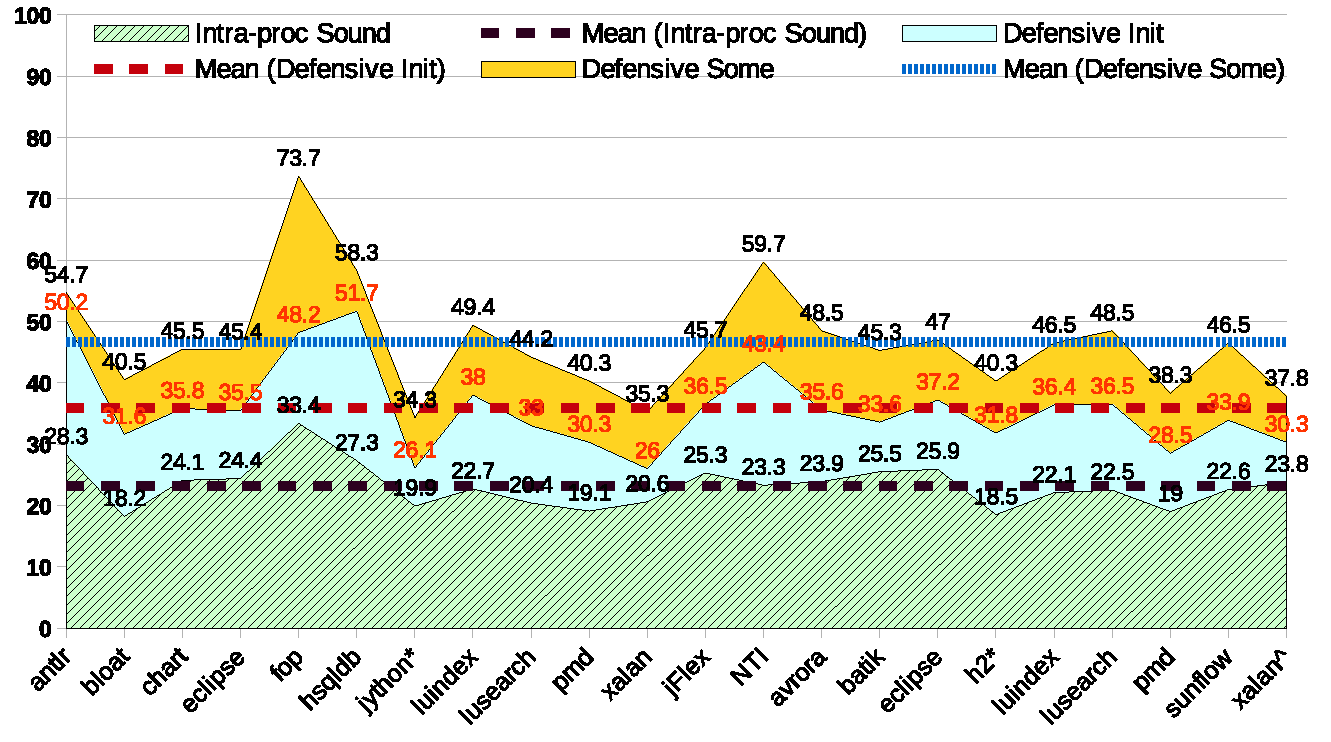
\includegraphics[width=\linewidth]{assets/defensive/vars.pdf}
  \end{minipage}
  \caption{Percentage of application variables (deemed reachable by
    baseline 2objH analysis) that have non-empty points-to sets for
    defensive analysis under some context and \textsc{Init} context (no
    assumptions). Intra-procedural sound points-to analysis (defensive
    minus the complex cases) shown as baseline. Arithmetic means are
    plotted as lines.}
    \label{fig:coverage}
\end{figure}

Thus, the defensive analysis achieves a large proportion of the
benefits of an unsound analysis, while guaranteeing these results
against uses of opaque code.  We can answer \textbf{RQ1}
affirmatively: defensive analysis covers a large part of realistic
programs (over one-third unconditionally; close to one half under
specific calling conditions), despite its conservative nature.

\paragraphhead{Comparison with intra-procedural.}
We have earlier referred to the ``easy'', intra-procedural parts of the
analysis reasoning: what a compiler or VM would likely do to perform
sound local data-flow analysis. This is the subject of \textbf{RQ2},
also answered by Figure~\ref{fig:coverage}. The figure includes
results for an intra-procedural baseline analysis that captures the
low-hanging fruit of sound reasoning: local variables that directly or
transitively (via ``move'' instructions) get assigned an allocated
object. That is, the ``Intra-proc Sound'' analysis is otherwise the
same as the full ``defensive'' logic, with the exception of the
new ``interesting'' cases (control-flow merging, heap manipulation,
and inter-procedural propagation). 

The result answers \textbf{RQ2} affirmatively: defensive analysis has
significantly higher coverage than the baseline intra-procedural
analysis. (And the difference only grows when considering an actual
client, in later experiments.) Although the benefit is not broken down
further in the figure, the handling of method calls alone (i.e., rules
\textsc{Call}, \textsc{Args} and \textsc{Ret}) is responsible for the
lion's share of the difference between the full defensive analysis and
the intra-procedural sound analysis.


%%% SPACE
%% Two data points in the experiment require further explanation. The
%% hsqldb benchmark is analyzed only partially by the underlying 2objH
%% analysis with the given reflection settings. Less than 10\% of the
%% statically available application code is deemed reachable.
%% % by 2objH, and is consequently also analyzed by 5def. 
%% The comparison of 2objH and 5def in this subset is still
%% meaningful, but may not be representative of the full complexity.
%% % of the hsqldb code. 
%% Also, for jython, 5def seems to cover 34.5\% of the application
%% variables produced by 2objH. However, this number is likely biased
%% (lowered) by the \emph{imprecision} of the unsound analysis: jython is
%% analyzed with a context-insensitive analysis, resulting in many
%% variables with spurious points-to sets.
%% % (See also later metrics on precision for jython.)
%% %
%% %If we allowed the 2objH
%% %analysis to complete (beyond a 3hr timeout) the real coverage of 5def
%% %would likely be higher for this benchmark. 

\paragraphhead{Running time.} 
Figure~\ref{fig:time} shows the running times of the analysis, plotted
next to that of 2objH, for reference.  Although the two analyses are
dissimilar, 2objH is qualitatively the closest one can get to
defensive analysis with the current state of the art: it is an
analysis with high precision, run with best-effort soundness
support. Therefore, 2objH can serve as a realistic point of reference.
As can be seen, the running times of defensive analysis are
realistically low, although its flow-sensitive and
5-call-site-sensitive nature suggests it would be a prohibitively
heavy analysis. This answers \textbf{RQ3} and confirms the benefits of
laziness: a defensive analysis that only populates points-to sets once
they are definitely bounded, achieves scalability for deep context.

\begin{figure}[tbhp]
  \begin{minipage}[b]{\linewidth}
    \centering
    % left bottom right top
    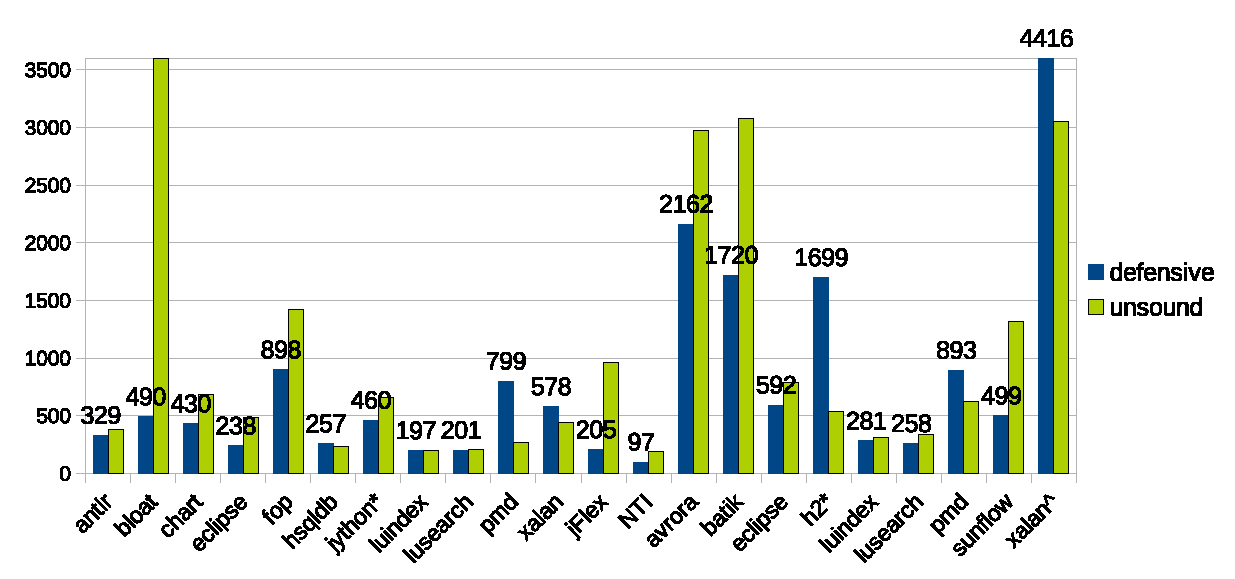
\includegraphics[width=\linewidth]{assets/defensive/time.pdf}
  \end{minipage}
  \caption{Running time (sec) of defensive analysis, with running time of
    2objH (with unsound reflection handling) shown as a
    baseline. Labels are shown for defensive analysis only to avoid
    crowding the plot.}
    \label{fig:time}
\end{figure}

%% As can be seen, 5def outperforms 2objH for
%% 16-of-22 benchmarks, one is tied, and 2objH is faster for 5 benchmarks
%% (also considering the 3 benchmarks for which either analysis timed out).

\paragraphhead{Client analysis: devirtualization.}
Our baseline analysis, 2objH, is highly precise and effective in
challenges such as devirtualizing calls (resolving virtual calls to a
single target method). On average, it can devirtualize 89.3\% of the
calls in the benchmarks studied (min: 78.5\%, max: 95.2\%). However,
these results are unsound and a compiler cannot act upon them. For
optimization clients, such as devirtualization, soundness is
essential. Using sound results, a JIT compiler can skip dynamic tests
(of the inline caching optimization) for all calls that the analysis
soundly covers.

Figure~\ref{fig:devirt1}
shows the virtual calls that defensive analysis devirtualizes, as a
percentage of those devirtualized by the unsound analysis.
\begin{figure}[tbhp]
  \begin{minipage}[b]{\linewidth}
    \centering
    % left bottom right top
    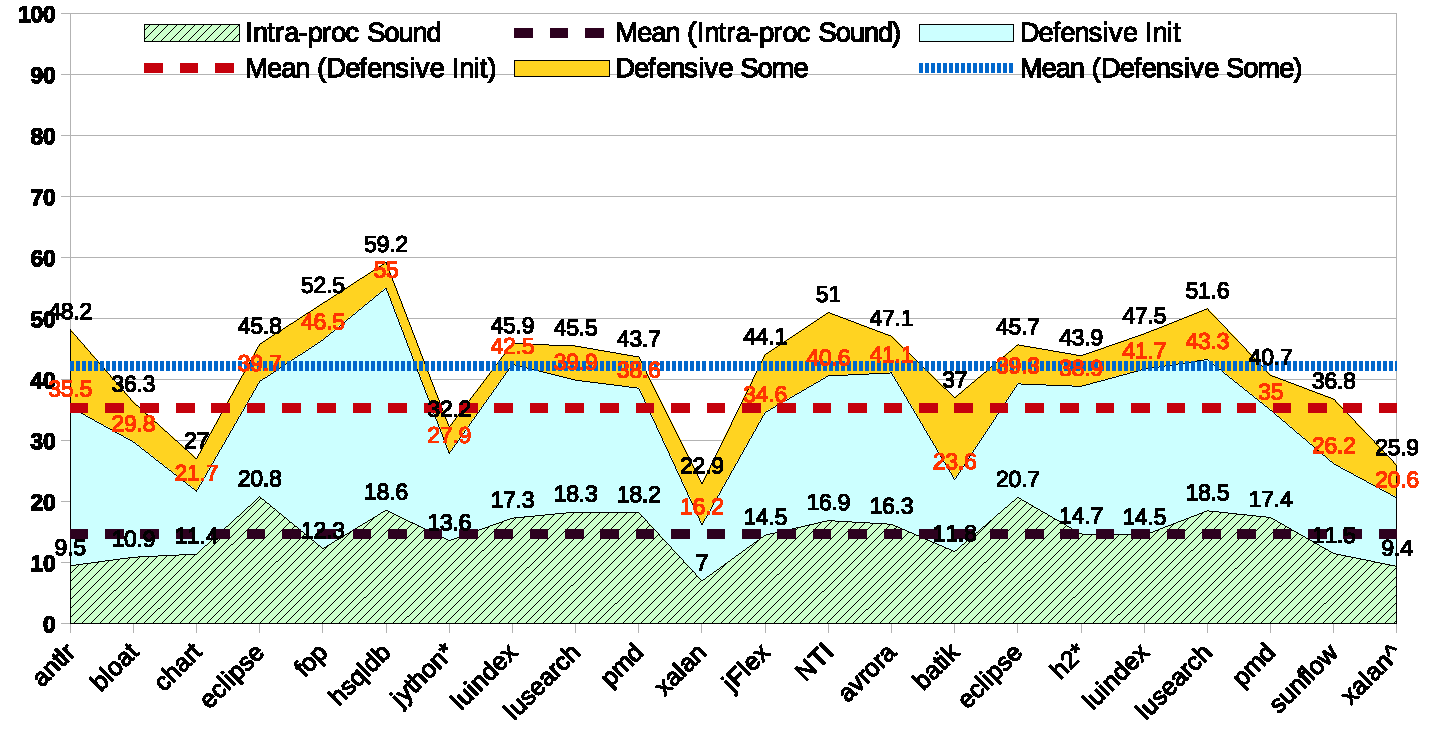
\includegraphics[width=\linewidth]{assets/defensive/devirt1.pdf}
  \end{minipage}
  \caption{Virtual call sites that are found to have receiver objects
    of a single type. These call sites can be soundly devirtualized.
    Numbers are shown as percentages of devirtualization achieved by
    unsound 2objH analysis.}
    \label{fig:devirt1}
\end{figure}

As can be
seen, defensive analysis manages to recover a large part of the
benefit of an unsound analysis (median \textbf{44.8\%} for
optimization under a context guard, \textbf{38.7\%} for unconditional,
\consname{Init} context, optimization), performing much better than
the baseline intra-procedural must-analysis (at 14.6\%). This answers
\textbf{RQ4} affirmatively: the coverage of defensive analysis translates
into real benefit for realistic clients.


\paragraphhead{Concurrency model.}
A compiler (JIT or AOT) author may (rightly) remark that the
concurrency model of Section~\ref{sec:assumptions} is not appropriate
for automatic optimizations. The Java concurrency model permits a lot
more relaxed behaviors, so the analysis is not sound for full Java as
stated. However, the benefit of defensive analysis is that it starts
from a sound basis and can add to it conservatively, only when it is
certain that soundness cannot possibly be violated. Accordingly, we
can remove the assumption that all shared data are accessed while
holding mutexes, by applying the load/store rules only when objects
trivially do not escape their allocating thread. We show the updated
numbers for the devirtualization client (now fully sound for Java!) in
Figure~\ref{fig:devirt2}. The difference in impact is minimal: \textbf{43\%} of
virtual call sites can be devirtualized conditionally, under some
context, while \textbf{36\%} can be devirtualized unconditionally. This
helps answer \textbf{RQ5}: defensive analysis can yield actionable results
for a well-known optimization, under the Java memory model, for a
large portion of realistic programs.

\begin{figure}[tbhp]
  \begin{minipage}[b]{\linewidth}
    \centering
    % left bottom right top
    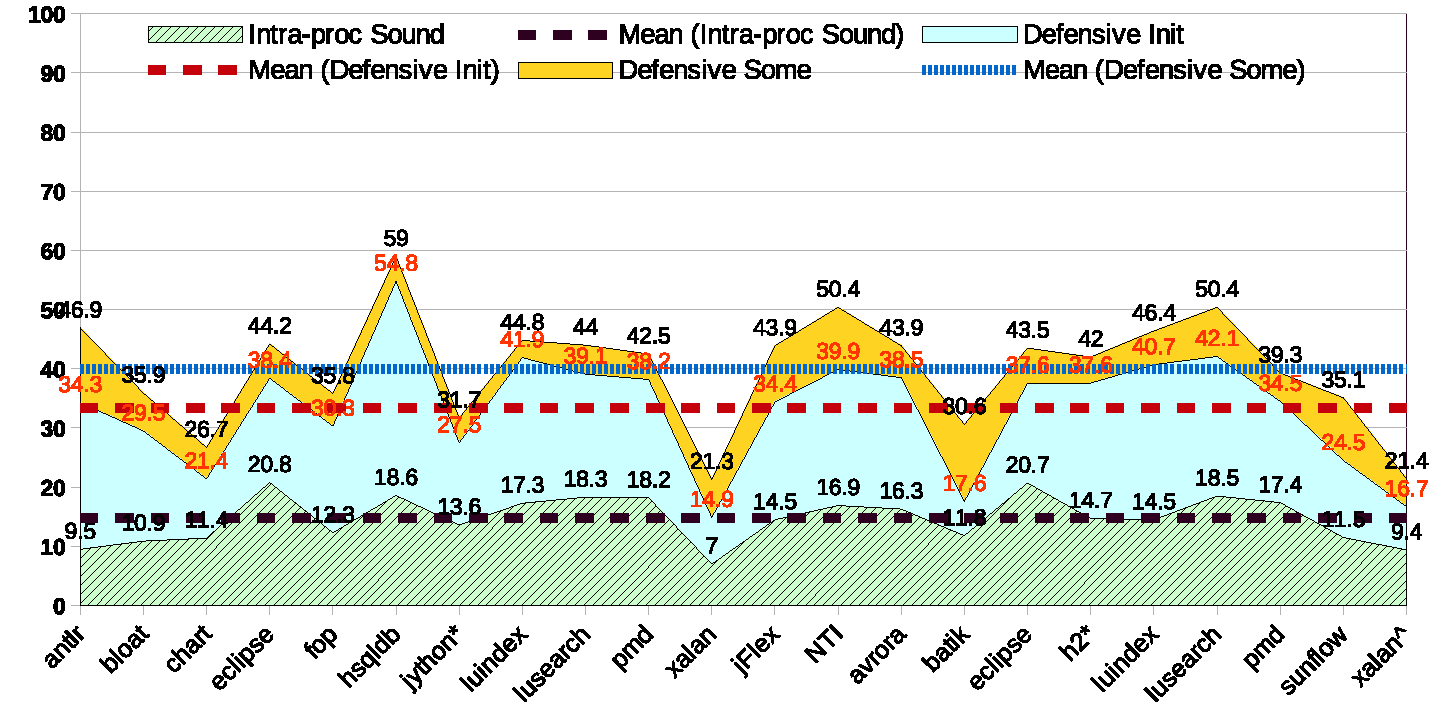
\includegraphics[width=\linewidth]{assets/defensive/devirt2.pdf}
  \end{minipage}
  \caption{Virtual call sites (percentage of 2objH) that are found to
    have receiver objects of a single type. Updates
    Figure~\ref{fig:devirt1}, this time with soundness under a relaxed
    memory model.}
   \label{fig:devirt2}
\end{figure}

\paragraphhead{Points-to set sizes.}
Finally, it is interesting to quantify the precision of the defensive
analysis, for the points-to sets it covers. This precision is expected
to be high, since defensive analysis is flow- and context-sensitive,
but exact figures help put it in perspective.

Figure~\ref{fig:precision} shows average points-to set sizes for the
defensive analysis vs. the 2objH analysis. The sets (excluding null
values) are computed over variables covered by both analyses, for
non-empty defensive analysis sets and under context \consname{Init}
of the defensive analysis, i.e., unconditionally. (The numbers are for
the simplistic concurrency model, but remain unchanged to two
significant digits for the relaxed concurrency model.)

%% The first comparison
%% (first two numeric columns) is over variables that the defensive
%% analysis covers for \emph{some} context, while the second (next two
%% columns) over variables that the defensive analysis covers for context
%% \consname{Init}. Again, the use of context in a defensive analysis is
%% different, so both numbers are biased, but in opposite ways. The
%% \emph{some context} comparison may exclude valid contexts for which
%% 5def computes empty sets, making it seem more precise. Conversely, the
%% \emph{Init context} numbers exclude variables whose points-to set
%% depends on method parameters, thus downplaying the
%% %precision 
%% impact of 5def's 5-call-site sensitivity. Still, the overall picture
%% is clear: 5def is highly precise.


%% \begin{figure}[t]
%% %  \small
%% \footnotesize
%%   \centering
%%    \begin{tabular}{lrrrr|rr}
%%     \toprule
%%     Bench. & \multicolumn{4}{c|}{Avg. points-to over same vars} & \multicolumn{2}{c}{Analysis time (s)} \\
%%   \midrule
%%            & \multirow{2}{2em}{\raggedleft 2objH {\footnotesize \emph{/ins.}}} & {\raggedleft 5def} & \multirow{2}{2.5em}{\raggedleft 2objH Init ctx} & \multirow{2}{2.5em}{\raggedleft 5def Init ctx} & \multirow{2}{2em}{\raggedleft 2objH {\footnotesize \emph{/ins.}}} & {\raggedleft 5def} \\
%% & & & & & & \\
%%     \midrule
%%     \midrule
%% antlr           &  1.55	 & 	1.13    & 1.10	 & 1.01   &  382   &  858  \\  
%% bloat           &  5.45	 & 	1.86    & 2.12	 & 1.02   &  4152  &  2045 \\
%% chart           &  1.37	 & 	1.29    & 1.09	 & 1.09   &  685   &  1644 \\
%% eclipse         &  1.81	 & 	1.17    & 1.31	 & 1.06   &  483   &  652  \\
%% hsqldb          &  1.09	 & 	1.04    & 1.04	 & 1.01   &  236   &  676  \\ 
%% jFlex           &  1.41  & 	1.19    & 1.02	 & 1.01   &  965   &  398  \\
%% \emph{jython*}  &  \emph{31.08} &  2.02    & \emph{6.05}	 & 1.01   &  \emph{655}   &  1435 \\ 
%% luindex         &  1.22	 & 	1.13    & 1.02	 & 1.02   &  197   &  562  \\
%% lusearch        &  1.35	 & 	1.21    & 1.06	 & 1.04   &  210   &  579  \\
%% NTI             &  1.47	 & 	1.43    & 1.03	 & 1.03   &  189   &  102  \\
%% xalan           &  2.55	 & 	1.77    & 1.12	 & 1.05   &  440   &  1152 \\
%%     \bottomrule
%%   \end{tabular}
%%   \caption{Points-to set sizes for non-empty sets of common variables for both analyses,
%%     and running times of analyses.}
%%   \label{fig:core}
%% \end{figure}

\begin{figure}[th!p]
%  \small
\footnotesize
  \centering
  \begin{tabular}{|cl|rr|}
    \toprule
    \multirow{2}{4em}{Benchmark}  & & \multicolumn{2}{c|}{Average points-to over same vars} \\
                   &             & defensive & 2objH  \\
  \midrule
  \midrule        
\multirow{11}{-0.2cm}{\rotatebox{90}{\footnotesize{\mbox{DaCapo 2006-10-MR2}}}} 
& antlr          & 1.01   &         1.10  \\
& bloat          & 1.02   &         2.12 	 \\
& chart          & 1.09   &         1.09 	 \\
& eclipse        & 1.06   &         1.31 	 \\
& fop            & 1.00   &         1.03 	 \\
& hsqldb         & 1.01   &         1.04   \\
& jython*        & 1.01   &         6.05 	 \\
& luindex        & 1.02   &         1.02   \\
& lusearch       & 1.04   &         1.06 	 \\
& pmd            & 1.01   &         1.05 	 \\
& xalan          & 1.05   &         1.12 	 \\
\midrule
& jFlex          & 1.01   &         1.02 	 \\
& NTI            & 1.03   &         1.03     \\
\midrule        
\multirow{9}{-0.2cm}{\rotatebox{90}{\footnotesize{\mbox{DaCapo 9.12-Bach}}}}
& avrora         & 1.05   &         3.04  \\
& batik          & 1.04   &         1.05 \\
& eclipse        & 1.07   &         1.53 \\
& h2*            & 1.04   &         2.07 \\
& luindex        & 1.01   &         1.04 \\
& lusearch       & 1.03   &         1.08 \\
& pmd            & 1.01   &         1.04 \\
& sunflow        & 1.05   &         1.08 \\
& xalan\^        & 1.04   &         1.19 \\
\midrule
& \textbf{mean} &   1.03     &  1.51  \\
    \bottomrule
  \end{tabular}
  \caption{Average number of abstract objects per variable, for variables for which both
    analyses compute results.}
  \label{fig:precision}
\end{figure}

As can be seen, the defensive analysis is highly precise when it produces non-empty
points-to sets, typically yielding points-to set sizes very close to
1. 2objH is also a very precise analysis (for variables with bounded
points-to sets), so it remains competitive, yet clearly less precise.
Notably, points-to set sizes close to 1 are the Holy Grail of points-to
analysis: such precision is actionable for nearly all conceivable clients
of a points-to analysis.


%% \begin{figure}[th!p]
%% %  \small
%% \footnotesize
%%   \centering
%%   \begin{tabular}{|cl|rrrr|}
%%     \toprule
%%     \multicolumn{2}{|l|}{\multirow{4}{4em}{Benchmark}} & \multirow{4}{5.5em}{\raggedleft App. calls devirtualized, 5def {\footnotesize \emph{($\dagger$4def)}} some context} & \multirow{3}{3em}{\raggedleft \% of 2objH {\footnotesize \emph{(*ins.)}}} & \multirow{4}{5.5em}{\raggedleft App. calls devirtualized, 5def {\footnotesize \emph{($\dagger$4def)}} \\ Init context} & \multirow{3}{3em}{\raggedleft \% of 2objH {\footnotesize \emph{(*ins.)}}}   \\
%%  & & & & & \\
%%  & & & & & \\
%%  & & & & & \\
%%   \midrule
%%   \midrule        
%% \multirow{11}{-0.2cm}{\rotatebox{90}{\footnotesize{\mbox{DaCapo 2006-10-MR2}}}} 
%% & antlr          & 7974     & 46.9\%   & 5825  & 34.3\% \\
%% & bloat          & 4821     & 35.9\%   & 3954  & 29.5\%	 \\
%% & chart          & 1022     & 26.7\%   & 820   & 21.4\%	 \\
%% & eclipse        & 2525     & 44.2\%   & 2191  & 38.4\%	 \\
%% & fop            & 764      & 35.8\%   & 645   & 30.3\%	 \\
%% & hsqldb         & 586      & 59.0\%   & 545   & 54.8\%  \\
%% & \emph{jython*} & 3623     & 31.7\%   & 3147  & 27.5\%	 \\
%% & luindex        & 930      & 44.8\%   & 870   & 41.9\%  \\
%% & lusearch       & 1055     & 44.0\%   & 939   & 39.1\%	 \\
%% & pmd            & 1876     & 42.5\%   & 1689  & 38.2\%	 \\
%% & xalan          & 1653     & 21.3\%   & 1155  & 14.9\%	 \\
%% \midrule
%% & jFlex          & 1190     & 43.9\%   & 933  &  34.4\%	 \\
%% & NTI            & 481      & 50.4\%   & 381  &  39.9\%    \\
%% \midrule        
%% \multirow{9}{-0.2cm}{\rotatebox{90}{\footnotesize{\mbox{DaCapo 9.12-Bach}}}}
%% & avrora         & 4564      & 43.9\%	 & 3996 & 38.5\%  \\
%% & batik          & 4404      & 30.6\%	 & 2527 & 17.6\% \\
%% & eclipse        & 2882      & 43.5\%    & 2490 & 37.6\% \\
%% & {\em h2*}      & 8452      & 42.0\%    & 7569 & 37.6\% \\
%% & luindex        & 2010      & 46.4\%    & 1761 & 40.7\% \\
%% & lusearch       & 1614      & 50.4\%    & 1349 & 42.1\% \\
%% & pmd            & 2262      & 39.3\%    & 1986 & 34.5\% \\
%% & sunflow        & 1114      & 35.1\%    & 780  & 24.5\% \\
%% & {\em xalan$\dagger$}& 4545 & 21.4\%	 & 3554 & 16.7\% \\
%% \midrule
%% & \textbf{median} &            &   43.0\%  &        &  36.0\%  \\
%%     \bottomrule
%%   \end{tabular}
%%   \caption{Virtual calls resolved to a single target method under relaxed concurrency model.}
%%   \label{fig:client2}
%% \end{figure}

%% \begin{figure}[t]
%% %  \small
%% \footnotesize
%%   \centering
%%    \begin{tabular}{lrrrr|rr}
%%     \toprule
%%     Bench. & \multicolumn{4}{c|}{Avg. points-to over same vars} & \multicolumn{2}{c}{Analysis time (s)} \\
%%   \midrule
%%            & \multirow{2}{2em}{\raggedleft 2objH {\footnotesize \emph{/ins.}}} & {\raggedleft 5def} & \multirow{2}{2.5em}{\raggedleft 2objH Init ctx} & \multirow{2}{2.5em}{\raggedleft 5def Init ctx} & \multirow{2}{2em}{\raggedleft 2objH {\footnotesize \emph{/ins.}}} & {\raggedleft 5def} \\
%% & & & & & & \\
%%     \midrule
%%     \midrule
%% antlr           &  1.55	 & 	1.13    & 1.10	 & 1.01   &  382   &  858  \\  
%% bloat           &  5.45	 & 	1.86    & 2.12	 & 1.02   &  4152  &  2045 \\
%% chart           &  1.37	 & 	1.29    & 1.09	 & 1.09   &  685   &  1644 \\
%% eclipse         &  1.81	 & 	1.17    & 1.31	 & 1.06   &  483   &  652  \\
%% hsqldb          &  1.09	 & 	1.04    & 1.04	 & 1.01   &  236   &  676  \\ 
%% jFlex           &  1.41  & 	1.19    & 1.02	 & 1.01   &  965   &  398  \\
%% \emph{jython*}  &  \emph{31.08} &  2.02    & \emph{6.05}	 & 1.01   &  \emph{655}   &  1435 \\ 
%% luindex         &  1.22	 & 	1.13    & 1.02	 & 1.02   &  197   &  562  \\
%% lusearch        &  1.35	 & 	1.21    & 1.06	 & 1.04   &  210   &  579  \\
%% NTI             &  1.47	 & 	1.43    & 1.03	 & 1.03   &  189   &  102  \\
%% xalan           &  2.55	 & 	1.77    & 1.12	 & 1.05   &  440   &  1152 \\
%%     \bottomrule
%%   \end{tabular}
%%   \caption{Points-to set sizes for non-empty sets of common variables for both analyses,
%%     and running times of analyses.}
%%   \label{fig:core}
%% \end{figure}

%\paragraphhead{Summary.}
%%The evaluation shows the great benefits of defensive
%%analysis (speed, precision)
%Defensive analysis offers speed and precision, while covering a
%non-trivial part of the program. The devirtualization client clearly
%demonstrates practical benefit.
%%of being sound.


%\afterpage{\FloatBarrier}







\section{Conclusions}

Static analysis has long suffered from unsoundness for perfectly
realistic language features, such as reflection, native code, or
dynamic loading. We presented a new analysis architecture that
achieves soundness by being \emph{defensive}. Despite its conservative
nature, the analysis manages to yield useful results for a large
subset of the code in realistic Java programs, while being efficient
and scalable. Additionally, the analysis is modular, as it can be
applied to any subset of a program and will yield sound results.

We expect this approach to open significant avenues for further
work. The analysis architecture can serve as the basis of other sound
analysis designs. The defensive analysis itself can be combined with
several other analyses (may-escape, must-alias) that have so far been
hindered by the lack of a sound substrate.
%The analysis can be enhanced with a wealth of
%extra information to extend its coverage.


%% \begin{figure*}[t]
%%   \small
%%   \centering
%%   \begin{tabular}{lrrrrrrrrrrrr}
%%     \toprule
%%     \multicolumn{13}{c}{\large \emph{Alias pairs}} \\
%%     % \cmidrule(l){2-13}
%%     \midrule
%%     & \multicolumn{3}{c}{intra-procedural}
%%     & \multicolumn{3}{c}{intra-procedural$^{+\text{may}}$}
%%     & \multicolumn{3}{c}{inter-procedural$_{-\text{may}}$}
%%     & \multicolumn{3}{c}{inter-procedural} \\
%%     \cmidrule(lr){2-4} \cmidrule(lr){5-7} \cmidrule(lr){8-10} \cmidrule(l){11-13}
%%     & \multirow{2}{2em}{per instr.} & \multirow{2}{3em}{\hfill per all-return} & time
%%     & \multirow{2}{2em}{per instr.} & \multirow{2}{3em}{per all-return} & time
%%     & \multirow{2}{2em}{per instr.} & \multirow{2}{3em}{per all-return} & time
%%     & \multirow{2}{2em}{per instr.} & \multirow{2}{3em}{per all-return} & time
%%     \\ Benchmark \\
%%     \midrule
%%     antlr    &  7 &  3 & 5m18s & 41 &  6 &  7m2s &  34 & 19 &  18m6s & 105 & 27 & 41m18s \\
%%     chart    & 10 &  4 & 5m58s & 15 &  6 & 5m55s &  26 & 20 &  7m52s & 34 & 24 &  9m18s \\
%%     luindex  &  4 &  3 & 2m27s &  7 &  6 & 2m50s &   7 &  7 &  3m17s & 12 & 12 &  3m25s \\
%%     lusearch &  5 &  3 & 2m51s &  6 &  5 & 2m52s &   8 &  6 &  3m20s & 12 & 10 &  3m54s \\
%%     pmd      & 13 &  3 & 5m44s & 15 &  4 & 5m37s &  23 & 17 & 11m17s & 27 & 19 & 12m57s \\
%%     \bottomrule
%%   \end{tabular}
%%   \caption{Average \#alias pairs per program element (with equivalent
%%     symmetric pairs removed, i.e., numbers divided by 2), and timings
%%     for various settings of the must-alias analysis.}
%%   \label{fig:exp1}
%% \end{figure*}



%\clearpage

%\renewcommand{\baselinestretch}{0.89}
%\renewcommand{\parsep}{0.2em}
%\bibliographystyle{super-abbrv}

%\bibliographystyle{abbrvnat}% \renewcommand{\bibfont}{\normalsize}
% \bibliography{cumulative-bib}

%%% Supplementary
%\begin{comment}


%% \appendix

%% \section{Soundness Proof}

%% We present informal but rigorous proofs of the main claims of our
%% analysis.

%% \subsection{Assumption/Guarantee Lemma}

%% We next discuss rules incrementally, with an eye towards establishing
%% their soundness. For each rule, we will present the soundness
%% \emph{assumptions} (preconditions) and \emph{guarantees}
%% (postconditions) it offers. We will later appeal to these properties
%% as a lemma in our soundness proof.

%% \paragraphhead{Initializing the analysis.}
%% The first rule initializes the analysis by making all
%% root methods reachable.

%% \begin{rules}
%% \rel{Reachable}{\consname{All}, meth} \rulearrow{} \relConf{RootMethod}{meth}.\\
%% \end{rules}

%% There are no soundness assumptions or guarantees for the above
%% rule. The input relation \relname{RootMethod} can contain arbitrary
%% contents and only affects the coverage of the analysis (since
%% otherwise points-to sets remain empty, i.e., implicitly
%% over-approximate).

%% \paragraphhead{Object allocation.} The 
%% handling of \relname{Alloc} instructions provides an unconditionally
%% sound points-to set. It is a base case for our inductive reasoning.

%% \begin{rules}
%% \rel{PointsTo}{i, ctx, \consapp{AP}{var}, heap} \rulearrow{} \\
%% \tab \rel{Alloc}{i, var, heap}, \rel{InMethod}{i, meth}, \\
%% \tab \rel{Reachable}{ctx, meth}. \\
%% \end{rules}

%% The rule computes an over-approximation of points-to sets \emph{per
%%   allocation instruction and its local variable}. (Other points-to
%% sets at the same program point---e.g., points-to sets carried over
%% from previous instructions---are not the responsibility of this rule,
%% so establishing their soundness is part of later reasoning.)

%% \myparagraph{Assumption:} the rule makes no assumptions on the state
%% of the computation before its firing.
%% % (Unlike later rules.) 

%% \myparagraph{Guarantee:} the rule produces over-approximate points-to
%% sets for all variables, \args{var}, that match in an execution of the
%% rule. This is easy to establish: at first, all points-to sets of such
%% \args{var}s are empty, i.e., denoting an implicitly over-approximate
%% value of $\top$. Once the rule executes and its body matches for a
%% certain allocation instruction \args{i}, the points-to set of the
%% variable assigned at \args{i} can only contain the freshly-allocated
%% object, \args{heap}, which is what the rule computes. No other program
%% instruction, in known or opaque code, can affect this
%% inference.\footnote{Recall that we assume an isolated heap and
%%   stack frames: no external code can affect local variables. We will
%%   use this assumption implicitly throughout.}

%% %\footnote{Recall our earlier warning about concurrency
%% %  models: we assume that all shared data accesses are
%% %  mutex-protected, so that no other thread can interfere with the
%% %  assignment. In Java-like languages, without an address-of operator
%% %  for local variables (such as the C/C++ \texttt{\&}), even this
%% %  assumption is unnecessary for this rule: local variable \args{var}
%% %  is guaranteed thread-local.}


%% \paragraphhead{Variable moves.} \relname{Move} instructions
%% can only produce sound sets if their input is sound.

%% \begin{rules}
%% \rel{PointsTo}{i, ctx, toAp, heap} \rulearrow{} \\
%% \tab \rel{Move}{i, to, from}, \\
%% \tab \rel{Before:PointsTo}{i, ctx, fromAp, heap}, \\
%% \tab \func{RebaseAP}{fromAp, from, to}{toAp}.\\
%% \end{rules}

%% \myparagraph{Assumption:} before execution of the rule, the points-to
%% set encoded in relation \relname{Before:PointsTo} (more precisely:
%% for every triple \args{i,ctx,fromAp} that matches the rule body in the
%% rule execution) is sound, i.e., it is either empty (to signify $\top$)
%% or contains all possible values that the access path may point to at
%% the given instruction and for any dynamic context matching the
%% analysis context. (In subsequent discussion we shall be less pedantic
%% in defining the points-to sets and values in question, since these are
%% easy to deduce in the context of a rule's explanation.)

%% \myparagraph{Guarantee:} The resulting points-to sets (encoded in
%% relation \relname{PointsTo}, for any \args{(i,ctx,toAp)} that match
%% in an execution of the rule) are sound, \emph{after full execution of
%%   the rule}. The latter is a subtle point, worth emphasizing, since it
%% is pervasive in our soundness reasoning.  Datalog rules induce
%% point-wise inferences. Our above rule refers to a single object,
%% \args{heap}, at a time, and not to the entire points-to set of
%% \args{fromAp} at once. Therefore, the rule's guarantee of soundness
%% only holds after the rule has been applied over the entire contents of
%% the relations in its body and all possible inferences have been
%% made. It is entirely possible that, during intermediate stages of the
%% rule's evaluation, points-to sets will be incomplete, i.e., neither
%% empty, nor containing all possible values. After full evaluation,
%% however, the soundness of the rule (under its earlier ``assumption''
%% on the input) is self-evident.


%% \paragraphhead{Heap loads.} Similarly, heap loads produce over-approximate
%% points-to sets if their input is also over-approximate.

%% \begin{rules}
%% \rel{PointsTo}{i, ctx, \consapp{AP}{to}, heap} \rulearrow{} \\
%% \tab \rel{Load}{i, to, base, fld}, \\
%% \tab \rel{Before:PointsTo}{i, ctx, \consapp{AP}{base.fld}, heap}.\\
%% \end{rules}

%% \myparagraph{Assumption:} As in the previous rule, before execution of
%% the rule, the points-to set encoded in relation
%% \relname{Before:PointsTo} should be sound (over-approximate), i.e.,
%% it is either empty or contains all possible values that an access path
%% may point to.

%% \myparagraph{Guarantee:} As before, the resulting points-to sets are
%% sound, after full execution of the rule (modulo concurrency models---recall
%% that we assume mutex-protected access to all shared data throughout).


%% \paragraphhead{Heap stores.} The next two rules handle writes to the heap
%% (store instructions).

%% \begin{rules}
%% \rel{PointsTo}{i, ctx, \consapp{AP}{base.fld}, heap} \rulearrow{} \\
%% \tab \rel{Store}{i, base, fld, from}, \\
%% \tab \rel{Before:PointsTo}{i, ctx, \consapp{AP}{from}, heap}.\\
%% \\
%% \rel{PointsTo}{i, ctx, ap, heap1},\\
%% \rel{PointsTo}{i, ctx, ap, heap2} \rulearrow{} \\
%% \tab \rel{Store}{i, base, fld, from}, \\
%% \tab \rel{Before:PointsTo}{i, ctx, \consapp{AP}{from}, heap1},\\
%% \tab \rel{Before:PointsTo}{i, ctx, ap, heap2},\\
%% \tab \args{ap} = \consapp{AP}{base'.fld}, \args{base} $\neq$ \args{base'}.\\
%% \end{rules}

%% \myparagraph{Assumption:} Before execution of the rule, the points-to
%% sets encoded in relation \relname{Before:PointsTo}, for any of the
%% involved access paths, should be sound (i.e., over-approximate).

%% \myparagraph{Guarantee:} As before, the resulting points-to sets are
%% sound, after full execution of the rule (modulo concurrency models).
%% To see this, consider that the second rule takes the union of the two
%% points-to sets (of \args{from} and of \args{ap}, both before the
%% instruction) as long as neither set is empty. At a store instruction,
%% there is nothing that can influence the contents of an object field,
%% other than its previous contents and the currently assigned value,
%% hence the rule is fully conservative.


%% \paragraphhead{Control-flow predecessors.} 
%% Next comes the rule for merging information from an instruction's
%% predecessors.

%% \begin{rules}
%% \rel{Before:PointsTo}{i, ctx, ap, heap} \rulearrow{} \\
%% \tab \rel{Next}{pred, i}, \\
%% \tab \rel{PointsTo}{pred, ctx, ap, heap},\\
%% \tab ($\forall$\args{j}: \rel{Next}{j, i} \ruleforall{} \rel{PointsTo}{j, ctx, ap, \_}).\\
%% \end{rules}

%% \myparagraph{Assumption:} Before execution of the rule, the points-to
%% sets encoded in relation \relname{PointsTo} should be sound, i.e.,
%% for each predecessor, the points-to set of \args{ap} at that
%% predecessor is either empty or contains all possible values that the
%% access path may point to.

%% \myparagraph{Guarantee:} The resulting points-to set is sound
%% (over-approximate), after full execution of the rule. This is easy to
%% establish by considering that the rule takes the union of all input
%% points-to sets (\relname{PointsTo} for \args{ap} at all predecessors)
%% as long as no single one of them is empty.
%% % (If even a single input
%% %points-to set for \args{ap} is empty, the rule does not match, hence
%% %the resulting points-to set is also empty, and not the union, as
%% %discussed in Section~\ref{sec:illustration}.)


%% \paragraphhead{Frame rules: before an instruction to after it.}
%% The next three rules state the
%% conditions under which points-to information can be kept unchanged by
%% an instruction.

%% \begin{rules}
%% \rel{PointsTo}{i, ctx, ap, heap} \rulearrow{} \\
%% \tab \rel{Before:PointsTo}{i, ctx, ap, heap}, \args{ap} = \consapp{AP}{var}, \\
%% \tab !\rel{Load}{i, var, \_, \_}, !\rel{Move}{i, var, \_}, \\
%% \tab !\rel{Alloc}{i, var, \_}, !\rel{Unknown}{i}.\\
%% \\
%% \rel{PointsTo}{i, ctx, ap, heap} \rulearrow{} \\
%% \tab \rel{Before:PointsTo}{i, ctx, ap, heap}, \args{ap} = \consapp{AP}{var.\_}, \\
%% \tab !\rel{Call}{i, \_, \_}, !\rel{Store}{i, \_, \_, \_}, !\rel{Load}{i, var, \_, \_}, \\
%% \tab !\rel{Move}{i, var, \_}, !\rel{Alloc}{i, var, \_}, !\rel{Unknown}{i}.\\

%% \\
%% \rel{PointsTo}{i, ctx, ap, heap} \rulearrow{} \\
%% \tab \rel{Store}{i, \_, fld, \_}, \\
%% \tab \rel{Before:PointsTo}{i, ctx, ap, heap}, \\
%% \tab \args{ap} = \consapp{AP}{\_.\_}, \args{ap} $\neq$ \consapp{AP}{\_.fld.\_}. \\
%% \end{rules}

%% \myparagraph{Assumption:} Before execution of each rule, the points-to
%% set for \args{ap} encoded in relation \relname{Before:PointsTo}
%% should be sound (over-approximate).

%% \myparagraph{Guarantee:} For each rule separately, the resulting
%% points-to set (in relation \relname{PointsTo}) is sound after full
%% execution of the rule. This requires some care to establish. First,
%% note that in our limited intermediate language (of 7 instructions
%% only) no instruction kind assigns a local variable, other than
%% \relname{Alloc}, \relname{Move} or \relname{Load}. (\relname{Call}
%% instructions cannot alter the value of local variables in their
%% callee, assuming call-by-value semantics and no pointers to local
%% variables, as discussed earlier.) Second, consider that the treatment
%% of \relname{Unknown} instructions is as conservative as it can
%% possibly be: all points-to information is dropped when an unknown
%% instruction is encountered. Finally, a potential complication arises
%% in that the applicability of these rules may overlap with the
%% applicability of earlier rules (or with each other). Inspection of all
%% cases (e.g., consider the above three rules and the two rules handling
%% heap store instructions) reveals that the body conditions of each frame
%% rule are mutually exclusive with the body conditions of earlier
%% rules or other frame rules.  

%% Therefore, a frame rule will either not be triggered, in which case
%% its output points-to set is empty (i.e., trivially over-approximate),
%% or will compute points-to sets for an access path \args{ap} after an
%% instruction \args{i}, such that \args{i} cannot have altered the points-to
%% set of \args{ap}. In the latter case, the (assumed over-approximate) points-to
%% set of \args{ap} from before the instruction is maintained and is, thus,
%% also over-approximate. 

%% The latter holds, again, modulo a concurrency model. Importantly,
%% our assumed model throughout this paper (shared data only accessed
%% while holding mutexes) is trivially handled by the above rules: a
%% mutex acquire instruction (e.g., a JVM \code{monitorenter}) is not
%% captured in our language, hence it is encoded as an ``unknown''
%% instruction.  Per the frame rules, this ensures that all points-to
%% information is prevented from propagating over a possible point of
%% interference from other threads.


%% \paragraphhead{Inter-procedural analysis: Over-approximate call-graph.}
%% Our next rule uses points-to information to establish a sound call-graph.

%% \begin{rules}
%% \rel{CallGraphEdge}{i, ctx, toMeth, toCtx}, \\
%% \rel{Reachable}{toCtx, toMeth} \rulearrow{} \\
%% \tab \rel{Call}{i, base, sig}, \\
%% \tab \rel{Before:PointsTo}{i, ctx, \consapp{AP}{base}, heap}, \\
%% \tab \rel{HeapType}{heap, type}, \rel{LookUp}{type, sig, toMeth}, \\
%% \tab \func{NewContext}{i, ctx, heap}{toCtx}.\\
%% \end{rules}

%% \myparagraph{Assumption:} Before execution of the rule, the points-to
%% set for \args{base} encoded in relation \relname{Before:PointsTo}
%% should be sound (over-approximate).

%% \myparagraph{Guarantee:} Relation \relname{CallGraphEdge} for
%% invocation site \args{i} encodes a sound call-graph for instruction
%% \args{i} under context \args{ctx}. Since \relname{Before:PointsTo}
%% over-approximates the receiver object for \args{(i,ctx)}, we also
%% derive (via type system lookup) an over-approximation of
%% the call targets (including empty as a trivial over-approximation).


%% \paragraphhead{Inter-procedural propagation of values: caller-to-callee.}

%% The next rule handles points-to information propagation over calls,
%% from caller to callee.

%% \begin{rules}
%% \rel{Before:PointsTo}{fstInstr, toCtx, ap, heap} \rulearrow{} \\
%% \tab \rel{CallGraphEdge}{i, ctx, toMeth, toCtx}, \\
%% \tab \rel{InMethod}{fstInstr, toMeth}, 
%%      ($\forall$\args{k}: \ruleforall{} !\rel{Next}{k, fstInstr}), \\
%% \tab \rel{Before:PointsTo}{i, ctx, callerAp, heap}, \\
%% \tab \rel{FormalArg}{toMeth, n, toVar}, \rel{ActualArg}{i, n, var}, \\
%% \tab \func{RebaseAP}{callerAp, var, toVar}{ap}.\\
%% \end{rules}

%% \myparagraph{Assumption:} Before execution of the rule, the points-to
%% sets encoded in relation \relname{Before:PointsTo} (for \args{base},
%% under \args{(i,ctx)} matching in the rule body) are over-approximate.

%% \myparagraph{Guarantee:} The points-to set computed (for \args{ap} at
%% instruction \args{fsInstr} under context \args{toCtx}) is
%% over-approximate, \emph{as long as the pair \args{(toMeth,toCtx)}
%%   uniquely identifies \args{i} and \args{ctx}}!  The latter is an
%% important restriction on the possible definitions of function
%% \consname{NewContext}. Rigorously speaking, we are trying to establish
%% that the set of \args{heap} values in \rel{Before:PointsTo}{fstInstr,
%%   toCtx, ap, heap} is over-approximate, given that
%% \rel{Before:PointsTo}{i, ctx, callerAp, heap} is. Values of variable
%% \args{fstInstr} map one-to-one to values of \args{toMeth}, and (given
%% invocation site \args{i} and target method \args{toMeth}) \args{ap}
%% maps one-to-one to \args{callerAp}. Hence, if the pair
%% \args{(toMeth,toCtx)} arises for only a single call site and caller
%% context pair, \args{(i,ctx)}, then the property clearly holds.  Recall
%% that this is our requirement for constructor \consname{NewContext}: it
%% should at least encode call-site sensitivity, i.e., the callee context
%% has to uniquely identify the call site.


%% \paragraphhead{Inter-procedural propagation of values: callee-to-caller.}
%% The next two rules perform a similar propagation of values, this time
%% from callee to caller. 
%% %A subtle difference from earlier is that the
%% %rule is predicated on having computed an over-approximation of the
%% %targets of a virtual call in relation \relname{CallGraphEdge}.
%% %(We
%% %did not need this assumption for propagation of points-to sets from
%% %caller to callee precisely because this information was predicated on
%% %context that uniquely identified the caller.)

%% \begin{rules}
%% \rel{RebaseAPForReturn}{i, ap, newAp} \rulearrow{} \\
%% \tab \rel{CallGraphEdge}{i, \_, toMeth, \_}, \\
%% \tab \rel{FormalArg}{toMeth, n, var}, \rel{ActualArg}{i, n, toVar}, \\
%% \tab \args{ap} = \consapp{AP}{\_.\_}, \func{RebaseAP}{ap, var, toVar}{newAp}.\\
%% \\
%% \rel{PointsTo}{i, ctx, ap, heap} \rulearrow{} \\
%% \tab \rel{CallGraphEdge}{i, ctx, toMeth, toCtx}, \\
%% \tab \rel{Return}{ret}, \rel{InMethod}{ret, toMeth}, \\
%% \tab \rel{Before:PointsTo}{ret, toCtx, calleeAp, heap}, \\
%% \tab \rel{RebaseAPForReturn}{i, calleeAp, ap}, \\
%% \tab ($\forall$\args{toMeth'}, \args{toCtx'}: \\
%% \tab \tab \rel{CallGraphEdge}{i, ctx, toMeth', toCtx'} \ruleforall{} \\
%% \tab \tab ($\exists$\args{ret'}, \args{calleeAp'}: \\
%% \tab \tab \tab \rel{Return}{ret'}, \rel{InMethod}{ret',toMeth'},  \\
%% \tab \tab \tab \rel{Before:PointsTo}{ret', toCtx', calleeAp', \_}, \\
%% \tab \tab \tab \rel{RebaseAPForReturn}{i, calleeAp', ap})). \\
%% \end{rules}

%% \myparagraph{Assumption:} Before execution of the rule, the points-to
%% sets encoded in relation \relname{Before:PointsTo} as well as the
%% call-graph encoded in \relname{CallGraphEdge} are
%% over-approximate.
%% %\footnote{Interestingly, we did not need the assumption
%% %that \relname{CallGraphEdge} be over-approximate for the case of
%% %propagating information from caller to callee, but we do for propagating
%% %information back from callee to caller. Intuitively, this continues our
%% %earlier remarks on how a defensive analysis only establishes points-to
%% %information at a callee conditionally, under a specific context that
%% %identifies the caller.}

%% \myparagraph{Guarantee:} The points-to set computed (for \args{ap} at
%% call-site \args{i}) is over-approximate. As in the case of store
%% instructions and control-flow merge points, the rule takes the union
%% of points-to sets for \args{ap} (suitably renamed) at all return
%% points (``all'' established by the soundness of
%% \relname{CallGraphEdge}), as long as not a single one of them is
%% empty. If any such points-to set is empty, the rule fails to match at
%% all, hence the overall resulting points-to set is empty.

%% It is worth noting that the handling of a method return is the only
%% point where a context can become stronger. Facts that were inferred to
%% hold under the more specific \args{toCtx} are now established, modulo
%% rebasing, under \args{ctx}.








%% \paragraphhead{Summary.}
%% This concludes the analysis model for our core intermediate language.
%% (There are many elements that can be added to the analysis to make it
%% more suitable for full languages and realistic programs. We postpone
%% the discussion of enhancements until Section~\ref{sec:discussion}.)  The
%% essence of the analysis is well-captured by this model. It is also
%% evident that the analysis has a strikingly different form from past
%% (unsound) points-to analyses in the literature. At every key point
%% (notably: control-flow merging, heap stores, inter-procedural
%% propagation of points-to sets) the analysis defensively ensures that
%% the information it has available is sufficient to establish an
%% upper-bounded points-to set, otherwise it reverts to computing an
%% empty set.




%% Reachable(ALL, meth) <-
%%    RootMethod(meth).

%% PointsTo(i, ctx, AP(var), heap) <-
%%    Alloc(i, var, heap),
%%    InMethod(i, meth),
%%    Reachable(ctx, meth).

%% PointsTo(i, ctx, toAp, heap) <-
%%    Move(i, to, from),
%%    Before:PointsTo(i, ctx, fromAp, heap),
%%    RebaseAP(fromAp, from, to) = toAp.

%% %PointsTo(i, ctx, toAp, heap) <-
%% %   Phi(i, _, _, ...),
%% %   (forall from: Phi(i, to, ..., from, ...) ->
%% %     Before:PointsTo(i, ctx, RebaseAP(toAp, to, from), heap)).

%% NewContext(i, ctx, heap) = toCtx,
%% CallGraphEdge(i, ctx, toMeth, toCtx),
%% Reachable(toCtx, toMeth) <-
%%    Call(i, base, sig),
%%    Before:PointsTo(i, ctx, AP(base), heap),
%%    HeapType(heap, type),
%%    LookUp(type, sig, toMeth).

%% ===============================

%% PointsTo(i, ctx, AP(to), heap) <-
%%    Load(i, to, base, fld),
%%    Before:PointsTo(i, ctx, AP(base.fld), heap).

%% PointsTo(i, ctx, AP(base.fld), heap) <-
%%    Store(i, base, fld, from),
%%    Before:PointsTo(i, ctx, AP(from), heap).

%% PointsTo(i, ctx, ap, heap1),
%% PointsTo(i, ctx, ap, heap2) <-
%%    Store(i, base, fld, from),
%%    Before:PointsTo(i, ctx, AP(from), heap1),
%%    Before:PointsTo(i, ctx, ap, heap2),
%%    ap = AP(base2.fld),
%%    base != base2.

%% %===============================
%% %// weakening
%% %
%% %PointsTo(i, ctx, ap, heap) <-
%% %   InMethod(i, meth),
%% %   Reachable(ctx, meth),
%% %   PointsTo(i, ALL, ap, heap).
%% %
%% %Before:PointsTo(i, ctx, ap, heap) <-
%% %   InMethod(i, meth),
%% %   Reachable(ctx, meth),
%% %   Before:PointsTo(i, ALL, ap, heap).
%% %
%% %===============================

%% // frame rules

%% Before:PointsTo(i, ctx, ap, heap) <-
%%    Next(pred, i), 
%%    PointsTo(pred, ctx, ap, heap),
%%    (forall j: Next(j, i) ->
%%       PointsTo(j, ctx, ap, _)).

%% PointsTo(i, ctx, ap, heap) <-
%%    Before:PointsTo(i, ctx, ap, heap),
%%    ap = AP(var),
%%    !Load(i, var, _, _),
%%    !Move(i, var, _),
%%    !Alloc(i, var, _),
%%    !Unknown(i).

%% PointsTo(i, ctx, ap, heap) <-
%%    Before:PointsTo(i, ctx, ap, heap),
%%    ap = AP(var._),
%%    !Call(i, _, _),
%%    !Store(i, _, _, _),
%%    !Unknown(i),
%%    !Load(i, var, _, _),
%%    !Move(i, var, _),
%%    !Alloc(i, var, _).

%% PointsTo(i, ctx, ap, heap) <-
%%    Before:PointsTo(i, ctx, ap, heap),
%%    ap = AP(_._),
%%    Store(i, _, fld, _),
%%    ap != AP(_.fld._).

%% ===============================

%% Before:PointsTo(firstInstr, toCtx, ap, heap) <-
%%    CallGraphEdge(i, ctx, toMeth, toCtx),
%%    InMethod(firstInstr, toMeth), (forall k -> !Next(k, firstInstr)),
%%    Before:PointsTo(i, ctx, callerAp, heap),
%%    FormalArg(toMeth, n, toVar), ActualArg(i, n, var),
%%    RebaseAP(callerAp, var, toVar) = ap.

%% RebaseAPForReturn(i, ap, newAp) <-
%%    CallGraphEdge(i, _, toMeth, _),
%%    FormalArg(toMeth, n, var), ActualArg(i, n, toVar), AP(_.fld) = ap,
%%    RebaseAP(ap, var, toVar) = newAp.

%% PointsTo(i, ctx, ap, heap) <-
%%    CallGraphEdge(i, ctx, toMeth, toCtx),
%%    Return(ret), InMethod(ret, toMeth), 
%%    Before:PointsTo(ret, toCtx, calleeAp, heap),
%%    RebaseAPForReturn(i, calleeAp, ap),
%%    (forall toMeth', toCtx' : CallGraphEdge(i, ctx, toMeth', toCtx') ->
%%       exist ret', calleeAp':
%%         Return(ret'), InMethod(ret', toMeth'),
%%         Before:PointsTo(ret', toCtx', calleeAp', _),
%%         RebaseAPForReturn(i, calleeAp', ap)).





%\end{comment}
%% Supplementary







\begin{comment}
\section{Why Is Sound Analysis Hard?}

In a recent article \cite{article:2015:Livshits}, Livshits et al. observe that
``\textit{[there is not] a single realistic whole-program analysis
  tool [...]  that does not purposely make unsound choices
  ... [V]irtually all published whole-program analyses are unsound and
  omit conservative handling of common language features when applied
  to real programming languages}''. 
%The sentiment echoes past
%observations, in more specific settings. For instance, Avots et
%al. \cite{icse/AvotsDLL05} remark: ``\textit{A C pointer alias
%  analysis cannot be strictly sound, or else it would conclude that
%  most locations in memory may point to any memory location.}''

Our defensive analysis addresses the above problems: the
analysis is sound as-specified (regardless of the extra features of
realistic programming languages) and yields realistic benefit. To
appreciate how the different architecture of our analysis solves the
problem, we need to first examine \emph{why} past analyses did not
manage to (or chose not to) be sound. (Our discussion focuses on
may-point-to analyses, but largely applies, with small adaptation, to
other static analyses.)

\paragraphhead{Observation: implicit over-approximation.}
A simple observation regarding a sound may-point-to analysis is that
points-to sets can only be \emph{implicitly} over-approximate. I.e.,
they cannot list exhaustively all the abstract objects that a variable
can point to, but instead should have catch-all values (such as
$\top$, as in traditional data-flow analysis) or marks (such as ``I''
for ``incomplete'' in past work \cite{pldi:2007:Lattner}).

To see this, consider the traditional explicit representation of
points-to sets in a static analysis. A set \code{\{o1, o3, o17\}}
includes abstract objects \code{o1}, \code{o3}, \code{o17}, which are
typically context-qualified allocation sites, i.e., program
instructions with some extra annotations. However, this representation
cannot capture objects allocated in \emph{unknown} code, such as
dynamically loaded code. 

Therefore a sound analysis (which needs to be over-approximate, i.e.,
to capture \emph{all} objects that a variable may point to during
\emph{any} execution) has to encode unknown objects implicitly, using
a special value.
%\footnote{Of course, an analysis can be sound by
%  computing an unknown, $\top$, value \emph{everywhere}, but such an
%  analysis will be obviously useless in practice.}  
Our defensive analysis also follows this pattern, yet the value
denoting that a points-to set is not completely known is
(unconventionally, but highly conveniently) the empty set.


\paragraphhead{Difficulty: non-monotonicity.} The first practical
difficulty of having a sound points-to analysis is the logical
non-monotonicity of inter-procedural (mainly heap-related) analysis
reasoning. To see the issue, consider the treatment of a standard
``load'' instruction from a heap object:

\vspace{-3mm}\begin{minipage}[l]{5.1in}
\begin{javacodeNoLines}
x = y.fld;
\end{javacodeNoLines}
\end{minipage}

\noindent For the analysis to upper-bound the set of values that
\code{x} may point to, it does not suffice to have upper-bounded the set
of values that \code{y} may point to and the values that \code{y}'s fields
may point to. Instead, it is necessary to know that \emph{every value
  pointed-to by \code{y} does not escape into opaque code}. For
instance, one possible value of \code{y} may be aliased, e.g., it may
also be known as \code{r.next.parent}, where \code{r} is a variable used
as a parameter to an opaque operation.  Thus, \code{x} can potentially
point to anything.

The above reasoning introduces a logical conundrum:

\begin{itemize}
\item To define a sound may-point-to analysis, we first need to have
  completed a sound \emph{may-escape} analysis, and take the
  complement of its results, in order to know what objects can \emph{never}
  escape into opaque code.
\item But, to define a sound (i.e., over-approximate) may-escape
  analysis, we first need to have a sound may-point-to analysis.
\end{itemize}

The above difficulty can be overcome, by introducing highly
conservative over-approximations of either a points-to or an escape
analysis, computing the other analysis based on the conservative
estimate, refining it, etc. In practice, this is a technical
complication. More importantly, it also implies that a large number of
objects can never be proven to not escape into opaque code. Listing
all such objects explicitly would be highly inefficient.\footnote{The
  only past analysis that attempts to do so is that of Lattner et
  al. \cite{pldi:2007:Lattner}, which has a special form that sidesteps the
  inefficiency at the expense of imprecision. The analysis employs a
  Steensgaard/unification-based analysis
  model~\cite{popl:1996:Steensgaard}. In this model, no
  object can belong in more than one points-to set, thus enabling a
  highly efficient representation of large sets of objects (using
  union-find trees), which cannot, however, be distinguished.} Note
that this also means that the special implicit object values discussed
earlier (such as $\top$) will necessarily represent not just
``unknown'' objects (i.e., in not-yet-loaded code) but also perfectly
normal objects that happen to escape into opaque code.
%This observation will come back to hurt us later.


\paragraphhead{Difficulty: capturing all opaque entry points and their
behavior.} Another difficulty of producing a sound analysis is
encoding all possible entry points into opaque code and their possible
behaviors. There are thousands of entry points into opaque code in a
realistic library (e.g., in the JDK). These include all native
methods, all reflection operations, \code{invokedynamic} instructions,
and more.  Furthermore, it is hard to model all behavior of these
entry points.  A single reflection operation can result in the leaking
of a large number of objects to a completely unforeseen method. Even
modeling reflection unsoundly (but with enough effort to have a
realistic treatment) faces a heavy engineering burden. For instance,
the latest reflection handling in the \textsc{Doop}
framework~\cite{aplas:2015:Smaragdakis} spans hundreds of logical
rules---a significant portion of the overall code base.

Even worse, the analysis needs to also model dynamically loaded code,
i.e., code that may not even exist at analysis time. It is far from
trivial to consider how dynamic loading can affect the analyzed
code---no past work has done so (except in very specific client
settings~\cite{pldi:2000:Sreedhar}---see
Section~\ref{sec:related}). The reason, again, has to do with
inter-procedural interactions. Extra code has the potential of
affecting nearly every inference of a whole-program analysis (e.g.,
static variables can almost always receive new values). It is easier
to compute what (and where) \emph{cannot} be influenced by
dynamically loaded code (i.e., to be defensive), than what \emph{can}.


\paragraphhead{Difficulty: wasting most work.} A sound points-to analysis
will likely be prohibitively expensive, due to the unpredictable order
of discovering what objects can be affected by opaque code.  Consider
our earlier example of a heap load, augmented with a virtual call,
inside a loop:
% and a back-edge in the control-flow:

\vspace{-3mm}\begin{minipage}[l]{5.1in}
\begin{javacode}
while (...) {
  x = y.fld;
  x.foo(y);
}
\end{javacode}
\end{minipage}

The analysis may well soundly compute all the object values that
\code{y} may point to at the load instruction (line 2). It may also have
computed the objects that \code{y.fld} object fields may point to. One
of these computed objects may induce a different resolution of the
call instruction (line 3), which can suddenly lead to the discovery
that a \code{y.fld}-aliased object can enter opaque code (while this was
not true based on what the analysis had computed earlier)! Since the
object referenced by \code{y.fld} can change in code that is not
analyzed, the points-to set of \code{x} at the load instruction will
need to be augmented with our implicit over-approximation special
value, $\top$.  This means that all previously computed values for the
points-to sets of \code{x} and \code{y.fld} are subsumed by the single
$\top$ value (which, recall, also represents regular objects that
escape into opaque code). Computing these values and all others that
depend on them constitutes wasted effort. To make matters worse, this
is more likely to happen for \emph{large} points-to sets, i.e., the
more work the analysis has performed on computing an explicit
points-to set, the larger (and less precise) the set will be, and the more
likely it is that the work will be wasted because the set will revert
to $\top$.

\end{comment}
